\باب{مقناطیسی قوتیں، مقناطیسی مادے اور امالہ}
برقی بار کے گرد برقی میدان پایا جاتا ہے جس میں موجود ساکن یا حرکت کرتے بار پر قوت دفع یا قوت کشش پایا جاتا ہے۔مقناطیسی میدان برقی رو یعنی حرکت کرتے بار سے پیدا ہوتا ہے اور اس میدان میں حرکت کرتے بار پر قوت پائی جاتی ہے۔مقناطیسی میدان ساکن بار پر قوت پیدا نہیں کرتا۔

اس باب میں برقی رو گزارتی تار پر قوت اور قوت گردشہ  کا جائزہ لیا جائے گا۔ اس کے بعد مقناطیسی اشیاء اور آخر میں\اصطلاح{ امالہ}\حاشیہب{inductance} پر غور کیا جائے گا۔

\حصہ{متحرک بار پر قوت}
تجربے سے  ثابت ہوتا ہے کہ برقی میدان میں بار بردار ذرے  پر 
\begin{align}\label{مساوات_امالہ_برقی_قوت}
\kvec{F}=Q \kvec{E}
\end{align}
قوت اثر انداز ہوتی ہے۔مثبت بار کی صورت میں یہ قوت برقی میدان کے شدت \عددیء{\kvec{E}} کی سمت میں ہوتی ہے۔قوت کی قیمت بار \عددیء{Q} اور برقی میدان کی شدت \عددیء{\kvec{E}} کے حاصل ضرب کے برابر ہوتی ہے۔بار ساکن ہو یا حرکت کر رہا ہو، اس پر قوت کی مقدار اسی مساوات سے حاصل ہوتی ہے۔

اسی طرح تجربے سے ثابت ہوتا ہے کہ مقناطیسی میدان میں ساکن بار بردار ذرے  پر مقناطیسی میدان کوئی قوت پیدا نہیں کرتا البتہ متحرک بار بردار ذرے  پر مقناطیسی میدان
\begin{align}\label{مساوات_امالہ_مقناطیسی_قوت}
\kvec{F}=Q \kvec{v} \times \kvec{B} 
\end{align}
قوت پیدا کرتا ہے۔یہ قوت بار  کے براہ راست متناسب ہوتی ہے۔اسی طرح قوت بار کے رفتار \عددیء{\kvec{v}}،  کثافت مقناطیسی میدان \عددیء{\kvec{B}} اور ان دو کے مابین زاویے کے سائن کے بھی براہ راست متناسب ہوتی ہے۔قوت کی سمت \عددیء{\kvec{v}} اور \عددیء{\kvec{B}} دونوں کے عمودی یعنی \عددیء{\kvec{v} \times \kvec{B}} سمت میں ہوتی ہے۔

مقناطیسی قوت رفتار کے عمودی ہے لہٰذا یہ رفتار کے قیمت پر اثر انداز نہیں ہوتا البتہ یہ اس کی سمت پر ضرور اثر ڈالتا ہے۔اس طرح مقناطیسی قوت بار بردار ذرے کے متحرک توانائی میں تبدیلی لانے سے قاصر ہے۔ اس کے برعکس برقی قوت جسے مساوات \حوالہ{مساوات_امالہ_برقی_قوت} بیان کرتا ہے بار بردار ذرے کی رفتار میں تبدیلی پیدا کرتے ہوئے حرکی توانائی میں تبدیلی پیدا کرتا ہے۔دونوں میدانوں میں یہ بنیادی فرق ہے کہ برقی میدان تبادلہ توانائی میں کردار ادا کرتا ہے جبکہ مقناطیسی میدان تبادلہ توانائی میں کردار ادا نہیں کرتا۔

دونوں میدانوں کے بیک وقت موجودگی میں بار بردار ذرے پر کل قوت
\begin{align}\label{مساوات_امالہ_لورنز}
\kvec{F}=Q\left(\kvec{E}+\kvec{v} \times \kvec{B} \right)
\end{align}
دونوں میدانوں سے علیحدہ علیحدہ پیدا قوتوں کے مجموعے کے برابر ہے۔مساوات \حوالہ{مساوات_امالہ_لورنز} \اصطلاح{لورنز مساوات قوت}\فرہنگ{لورنز مساوات قوت}\حاشیہد{یہ مساوات ہینڈرک لورنز کے نام ہے۔}\حاشیہب{Lorentz force equation}\فرہنگ{Lorentz force equation} کہلاتی ہے۔برقی اور مقناطیسی میدانوں میں بار بردار ذرے، مثلاً الیکٹران، کے راہ اسی مساوات کو حل کرتے ہوئے حاصل کئے جاتے ہیں۔
%===========

\ابتدا{مشق}
ایک عدد نقطہ بار جس کی قیمت \عددیء{\SI{-3}{\coulomb}} اور رفتار \عددیء{\kvec{v}=2\ax-3\ay+\az} ہو پر مندرجہ ذیل میدانوں میں قوت کی حتمی قیمت حاصل کریں۔
(الف) \عددیء{\kvec{E}=3\ax-2\ay-5\az}، (ب) \عددیء{\kvec{B}=-2\ax-3\ay+6\az}، (پ) دونوں میدانوں کے بیک وقت موجودگی میں۔

جوابات:\عددی{\SI{18.49}{\newton}}،  \عددی{\SI{71.3}{\newton}}، \عددی{\SI{78.7}{\newton}}
\انتہا{مشق}
%=====================

\حصہ{تفرقی بار پر قوت}
مقناطیسی میدان میں متحرک تفرقی بار \عددیء{\dif Q} پر تفرقی قوت \عددیء{\dif \kvec{F}} عمل کرے گی۔  
\begin{align}\label{مساوات_امالہ_مقناطیسی_تفرقی_قوت}
\dif \kvec{F}=\dif Q \kvec{v} \times \kvec{B}
\end{align}

آپ جانتے ہیں کہ منفی بار کی باریک ترین مقدار الیکٹران کا بار ہے۔مثبت بار کی باریک ترین قیمت بھی اتنی ہی لیکن مثبت قطب کی ہے۔منفی بار کو مثال بناتے ہوئے، یوں مندرجہ بالا مساوات میں تفرقی بار سے مراد کم از کم اتنا بار ہے جس میں الیکٹرانوں کی تعداد اتنی ہو کہ کسی ایک الیکٹران کے بار کا اثر قابل نظر انداز ہو۔اسی طرح اس تفرقی بار کا حجم اگرچہ چھوٹا ہے لیکن اس حجم کی جسامت الیکٹرانوں کے مابین اوسط فاصلے سے بہت زیادہ ہے۔مساوات \حوالہ{مساوات_امالہ_مقناطیسی_تفرقی_قوت} تفرقی بار پر کل قوت دیتا ہے۔یہاں یہ سمجھ لینا ضروری ہے کہ یہ قوت کسی ایک الیکٹران پر اثر انداز نہیں ہوتا بلکہ یہ تمام الیکٹرانوں پر علیحدہ علیحدہ قوتوں کا مجموعہ ہے۔ 

موصل تار میں برقی رو، الیکٹران کے حرکت کی بدولت ہے۔برقی رو گزارتے تار کو مقناطیسی میدان میں رکھنے سے تار میں ہر الیکٹران پر مقناطیسی قوت کا اثر پایا جائے گا۔اگرچہ کسی ایک الیکٹران پر انتہائی کم قیمت کا قوت پایا جاتا ہے لیکن موصل تار میں الیکٹرانوں کی تعداد انتہائی زیادہ ہوتی ہے۔یوں انتہائی زیادہ تعداد میں انتہائی کم قوتوں کا مجموعہ معقول قیمت کی قوت پیدا کرتا ہے۔آئیں دیکھتے ہیں کہ یہ مجموعی قوت تار تک کس طرح منتقل ہوتی ہے۔

موصل میں مثبت ایٹم یا آئن ساکن ہوتے ہیں جبکہ الیکٹران آزادی سے حرکت کر سکتے ہیں۔مقناطیسی میدان میں برقی رو گزارتے موصل تار میں حرکت پذیر منفی الیکٹران پر مقناطیسی قوت عمل کرتی ہے جس سے مثبت آئن اور منفی الیکٹران کے مابین فاصلوں میں تبدیلی رونما ہوتی ہے۔اب مثبت اور منفی بار کے مابین کولمب قوتیں ایسی تبدیلی کو روکتے ہیں لہٰذا حرکت پذیر الیکٹران پر مقناطیسی قوت یوں ساکن آئن تک پہنچ پاتی ہیں جو بطور تار پر مقناطیسی قوت کی صورت میں رونما ہوتی ہے۔

\begin{figure}
\centering
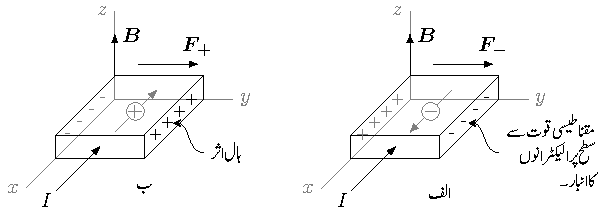
\includegraphics{figInductanceHallEffect}
\caption{ہال اثر سے متحرک بار کا قطب دریافت کیا جا سکتا ہے۔}
\label{شکل_امالہ_ہال_قطب_کا_حصول}
\end{figure}

مثبت آئن اور منفی الیکٹران کے مابین کولمب قوتیں انتہائی طاقتور ہوتی ہیں لہٰذا مقناطیسی میدان سے پیدا فاصلوں میں تبدیلی قابل ناپ نہیں ہوتی۔مثبت اور منفی باروں کے مابین فاصلے کی بنا پر انہیں دو چادر برق گیر  تصور کیا جا سکتا ہے۔ہم جانتے ہیں کہ ایسے برق گیر  کے چادروں کے مابین برقی دباو پایا جاتا ہے۔یوں الیکٹران کے حرکت اور مقناطیسی میدان دونوں کی سمتوں کے عمودی دو الٹ اطراف کے مابین تار پر معمولی برقی دباو پایا جاتا ہے جسے \اصطلاح{ہال اثر}\فرہنگ{ہال!اثر}\حاشیہب{Hall effect}\فرہنگ{Hall!effect} کے نام\حاشیہد{ایڈون حال نے اس اثر کو  1879 میں دریافت کیا۔} سے جانا جاتا ہے۔

ہال اثر کو شکل \حوالہ{شکل_امالہ_ہال_قطب_کا_حصول} کی مدد سے باآسانی سمجھا جا سکتا ہے۔شکل-الف میں موصل یا \عددیء{n} قسم کے نیم موصل برقی رو گزارتا تار دکھایا گیا ہے۔تار میں برقی رو \عددیء{I} کی سمت \عددیء{-\ax} ہے  لہٰذا تار میں آزاد منفی بار اس کے الٹ یعنی \عددیء{\ax} سمت  میں حرکت کر رہے ہیں۔تار میں آزاد الیکٹران کو ہلکی سیاہی میں تیر کے نشان پر دائرے میں بند \عددیء{-} علامت سے ظاہر کیا گیا ہے جہاں تیر اس کے حرکت کی سمت ظاہر کرتا ہے۔یہ تار \عددیء{\az} سمت کے مقناطیسی میدان میں پڑی ہے۔تار میں آزاد بار منفی قطب کے ہیں لہٰذا ان پر مساوات \حوالہ{مساوات_امالہ_مقناطیسی_قوت} کے تحت \عددیء{\ay} سمت میں قوت \عددیء{\kvec{F_-}} عمل کرے گا۔قوت کی علامت پر زیر نوشت میں منفی کی علامت یہ ظاہر کرتی ہے کہ یہ قوت متحرک منفی بار پر اثر انداز ہوتا ہے۔یوں تار کے دائیں طرف پر منفی الیکٹرانوں کا انبار جمع ہوتا ہے جبکہ تار کے بائیں طرف پر الیکٹران کی تعداد کم ہو جاتی ہے جس سے اس جانب ساکن مثبت آئن \اصطلاح{بے پردہ}\فرہنگ{بے پردہ}\حاشیہب{uncovered}\فرہنگ{charges!uncovered} ہو جاتے ہیں۔شکل \حوالہ{شکل_امالہ_ہال_قطب_کا_حصول}-الف میں تار کے دائیں طرف \عددیء{-} اور بائیں طرف  \عددیء{+} کے علامات انہیں کو ظاہر کرتے ہیں۔آپ جانتے ہیں کہ مثبت اور  منفی بار  کے مابین برقی میدان کی شدت \عددیء{\kvec{E}} اور یوں برقی دباو پایا جاتا ہے لہٰذا تار کے دائیں اور بائیں اطراف کے مابین \اصطلاح{ہال برقی دباو}\فرہنگ{ہال!برقی دباو}\حاشیہب{Hall voltage}\فرہنگ{Hall!voltage} پایا جائے گا۔تار کا بایاں طرف ہال برقی دباو کا مثبت سرا ہو گا۔

آئیں ایسی صورت دیکھیں جہاں متحرک مثبت بار کی بدولت برقی رو پائی جائے۔شکل \حوالہ{شکل_امالہ_ہال_قطب_کا_حصول}-ب میں بقایا صورت حال بالکل شکل-الف کی طرح ہے البتہ یہاں تار \عددیء{p} قسم کے نیم موصل کا بنا ہوا ہے جس میں برقی رو مثبت \اصطلاح{آزاد خول}\فرہنگ{خول!آزاد}\حاشیہب{free holes}\فرہنگ{holes!free} کے حرکت سے پیدا ہوتی ہے۔یوں اگر برقی رو \عددیء{-\ax} سمت میں ہو تب آزاد خول بھی اسی سمت میں حرکت کریں گے۔جیسے شکل میں دکھایا گیا ہے یہاں بھی مقناطیسی قوت آزاد بار کو دائیں جانب دھکیل رہے ہیں۔آپ دیکھ سکتے ہیں کہ اس مرتبہ ہال برقی دباو کا مثبت سرا تار کا دائیں طرف پایا جاتا ہے جو شکل-الف کے عین الٹ ہے۔اس حقیقت کو استعمال کرتے ہوئے یہ معلوم کیا جا سکتا ہے کہ آیا  نیم موصل \عددیء{n} یا \عددیء{p} قسم کا ہے۔

ہال اثر استعمال کرتے ہوئے مختلف پیمائشی آلات بنائے جاتے ہیں مثلاً \اصطلاح{یک سمتی رو پیما}\فرہنگ{ہال!یک سمتی رو پیما}\فرہنگ{Hall!effect current meter}، \اصطلاح{مقناطیسی بہاو پیما}\فرہنگ{ہال!مقناطیسی بہاو پیما}\حاشیہب{magnetic flux meter}\فرہنگ{Hall!magnetic flux meter} وغیرہ۔

سمتی رفتار \عددیء{\kvec{v}} سے حرکت کرتا ہوا حجمی کثافت بار \عددیء{\rho_h}  کثافت برقی رو \عددیء{\kvec{J}}
\begin{align}
\kvec{J}=\rho_h \kvec{v}
\end{align}
کو جنم دیتا ہے۔اس مساوات کو صفحہ \حوالہصفحہ{مساوات_کپیسٹر_کثافت_رو_مساوی_کثافت_بار_ضرب_رفتار} پر حاصل کیا گیا۔چھوٹے حجم \عددیء{\dif h} میں تھوڑے سے بار کو
\begin{align}
\dif Q=\rho_h \dif h
\end{align}
لکھا جا سکتا ہے لہٰذا مساوات \حوالہ{مساوات_امالہ_مقناطیسی_تفرقی_قوت} کو
\begin{align*}
\dif \kvec{F}=\rho_h \dif h \kvec{v} \times \kvec{B}
\end{align*}
یا
\begin{align}\label{مساوات_امالہ_لورنز_تفرقی_الف}
\dif \kvec{F}=\kvec{J} \times \kvec{B} \dif h
\end{align}
لکھا جا سکتا ہے۔ہم مساوات \حوالہ{مساوات-مقناطیسی_تفرقی_برقی_رو_مختلف_صورت} میں دیکھ چکے ہیں کہ \عددیء{\kvec{J} \dif h} کو برقی رو گزارتے تار کا تفرقی حصہ تصور کیا جا سکتا ہے جسے 
\begin{align*}
\kvec{J} \dif h=\kvec{K} \dif S=I \dif \kvec{L}
\end{align*}
بھی لکھا جا سکتا ہے۔اس طرح مساوات \حوالہ{مساوات_امالہ_لورنز_تفرقی_الف} کو
\begin{align}\label{مساوات_امالہ_لورنز_تفرقی_ب}
\dif \kvec{F}=\kvec{K} \times \kvec{B} \dif S
\end{align}
یا 
\begin{align}\label{مساوات_امالہ_لورنز_تفرقی_پ}
\dif \kvec{F}=I \dif \kvec{L} \times \kvec{B}
\end{align}
بھی لکھا جا سکتا ہے۔

مساوات \حوالہ{مساوات_امالہ_لورنز_تفرقی_الف}، مساوات \حوالہ{مساوات_امالہ_لورنز_تفرقی_ب} اور مساوات \حوالہ{مساوات_امالہ_لورنز_تفرقی_پ} کے تکمل سے انہیں یوں
\begin{align}
\kvec{F}&=\int_h \kvec{J} \times \kvec{B} \dif h \label{مساوات_امالہ_لورنز_تکمل_ت}\\
\kvec{F}&=\int_S \kvec{K} \times \kvec{B} \dif S \label{مساوات_امالہ_لورنز_تکمل_ٹ}\\
\kvec{F}&=\oint I \dif \kvec{L} \times \kvec{B} \label{مساوات_امالہ_لورنز_تکمل_پ}
\end{align}
لکھا جا سکتا ہے۔

مساوات \حوالہ{مساوات_امالہ_لورنز_تکمل_پ} میں اگر سیدھی تار لی جائے جس کی لمبائی \عددیء{L} ہو  تو تکمل سے
\begin{align}\label{مساوات_امالہ_سیدھی_تار_قوت_الف}
\kvec{F}=I \kvec{L} \times \kvec{B}
\end{align}
حاصل ہوتا ہے جس میں قوت کی قیمت
\begin{align}\label{مساوات_امالہ_سیدھی_تار_قوت_ب}
F=I L B \sin \alpha
\end{align}
ہے جہاں تار اور مقناطیسی میدان کے درمیان زاویہ \عددیء{\alpha} ہے۔مساوات \حوالہ{مساوات_امالہ_سیدھی_تار_قوت_الف} اور مساوات \حوالہ{مساوات_امالہ_سیدھی_تار_قوت_ب} پورے دور کے کچھ حصے پر قوت دیتے ہیں۔دور کے بقایا حصوں پر بھی اسی طرح قوت حاصل کئے جا سکتے ہیں۔

%=====================
\ابتدا{مثال}
محدد \عددی{z} پر لامحدود لمبائی کی تار میں \عددی{\SI{1.5}{\ampere}} کی برقی رو \عددی{\az} جانب گزر رہی ہے۔اس کے قریب نقطہ \عددی{N_1(3,2,5)} تا
 \عددی{N_2(4,6,1)} کے درمیان سیدھی موصل تار میں \عددی{\SI{2.3}{\ampere}} کی برقی رو \عددی{N_1} سے \عددی{N_2} کی جانب گزر رہی ہے۔اس تار پر مقناطیسی قوت حاصل کریں۔

حل:پہلی تار مقناطیسی میدان 
\begin{align*}
\kvec{B}&=\frac{1.5 \mu_0}{2\pi \rho}\aphi\\
&=\frac{1.5\mu_0}{2\pi \sqrt{x^2+y^2}}\left(-\frac{y}{\sqrt{x^2+y^2}}\ax+\frac{x}{x^2+y^2}\ay\right)\\
&=\frac{1.5\mu_0}{2\pi(x^2+y^2)}(-y\ax+x\ay)
\end{align*}
پیدا کرتا ہے جو دوسری تار کے چھوٹے حصے \عددی{\dif \kvec{L}=\dif x \ax+\dif y \ay+\dif z \az} پر قوت
\begin{align}\label{مثال_امالہ_ترچھی_تار}
\dif \kvec{F}=2.3 \dif \kvec{L} \times \kvec{B}
\end{align} 
پیدا کرے گی۔تار کی مساوات \عددی{\kvec{L}=x\ax+y\ay+z\az} میں \عددی{x}، \عددی{y} اور \عددی{z} متغیرات کو ایک ہی متغیرہ \عددی{t} کی صورت میں یوں لکھا جا سکتا ہے۔
\begin{align*}
x&=3+(4-3)t=3+t\\
y&=2+(6-2)t=2+4t\\
z&=5+(1-5)t=5-4t
\end{align*}
جہاں \عددی{t=0} پر کرنے سے ابتدائی نقطہ \عددی{N_1(3,2,5)} اور \عددی{t=1} پر کرنے سے اختتامی نقطہ \عددی{N_2(4,6,1)} حاصل ہوتا ہے۔یوں
\begin{align*}
\kvec{L}=(3+t)\ax+(2+4t)\ay+(5-4t)\az
\end{align*}
لکھ کر \عددی{\dif \kvec{L}=\dif t \ax+4\dif t \ay-4\dif t \az} لکھا جا سکتا ہے۔اس طرح پوری تار پر قوت مساوات \حوالہ{مثال_امالہ_ترچھی_تار} کے تکمل سے یوں 
\begin{align*}
\kvec{F}&=\int_0^1 2.3 ( \ax+4\ay-4 \az)\dif t \times \frac{1.5\mu_0}{2\pi[(3+t)^2+(2+4t)^2]}[-(2+4t)\ax+(3+t)\ay]\\
&=\int_0^1 \frac{3.45\mu_0}{2\pi(17t^2+22t+13)}[4(t+3)\ax+8(2t+1)\ay+(17t+11)\az]\dif t
\end{align*}
لکھی جا سکتی ہے جس سے
\begin{align*}
\kvec{F}=369\ax+386\ay+478\az \, \si{\nano\newton}
\end{align*}
حاصل ہوتا ہے۔
\انتہا{مثال}
%=============================
\حصہ{برقی رو گزارتے تفرقی تاروں کے مابین قوت}
شکل میں نقطہ \عددیء{N_1} پر تار کا ایک چھوٹا ٹکڑا \عددیء{\dif \kvec{L}_1} دکھایا گیا ہے جس میں \عددیء{I_1} برقی رو گزر رہی ہے  جبکہ نقطہ \عددیء{N_2} پر تار کا دوسرا چھوٹا ٹکڑا \عددیء{\dif \kvec{L}_2} دکھایا گیا ہے جس میں \عددیء{I_2} برقی رو گزر رہی ہے۔ نقطہ \عددیء{N_2} پر تار کے پہلے ٹکڑے سے پیدا مقناطیسی میدان مساوات \حوالہ{مساوات_بایوٹ_سیوارٹ_تفرق_شکل_ب} دیتا ہے۔

\begin{align*}
\dif \kvec{H}_2&=\frac{I_1 \dif \kvec{L}_1 \times \kvec{a}_{R21}}{4 \pi R_{21}^2}
\end{align*}
مساوات \حوالہ{مساوات_امالہ_لورنز_تفرقی_پ} مقناطیسی میدان \عددیء{\kvec{H}_2} میں تار کے تفرقی حصے پر تفرقی قوت دیتا ہے۔تفرقی مقناطیسی میدان \عددیء{\dif \kvec{H}_2} سے \عددیء{\dif \kvec{L}_2} پر  پیدا قوت درکار ہے۔اس قوت کو تفرقی قوت کا تفرقی حصہ \عددیء{\dif(\dif \kvec{F}_2)} لکھتے ہوئے مساوات \حوالہ{مساوات_امالہ_لورنز_تفرقی_پ} کو 
\begin{align*}
\dif \left(\dif \kvec{F}_2 \right)=I_2 \dif \kvec{L}_2 \times \dif \kvec{B}_2
\end{align*}
لکھا جا سکتا ہے جہاں \عددیء{\dif \kvec{B}_2=\mu_0 \dif \kvec{H}_2} کے برابر ہے۔مندرجہ بالا دو مساوات سے درج ذیل حاصل ہوتا ہے۔
\begin{align}\label{مساوات_امالہ_تفرقی_تفرقی_قوت}
\dif \left(\dif \kvec{F}_2 \right)=\mu_0 \frac{I_1 I_2}{4\pi R_{21}^2} \dif \kvec{L}_2 \times \left(\dif \kvec{L}_1 \times \kvec{a}_{R21} \right)
\end{align}
یاد رہے کہ کسی بھی نقطے پر برقی رو سے پیدا مقناطیسی میدان حاصل کرتے وقت ضروری ہے کہ پورے تار پر تکمل حاصل کیا جائے۔مندرجہ بالا مساوات میں نقطہ \عددیء{N_2} پر مکمل تکمل لیتے ہوئے میدان \عددیء{\kvec{H}_2} استعمال نہیں کیا گیا بلکہ تفرقی میدان \عددیء{\dif \kvec{H}_2} استعمال کیا گیا ہے۔یوں اگر اس مساوات سے قوتیں حاصل کی جائیں تو یہ درست نہیں ہوں گی۔یہ دیکھنے کے لئے تصور کریں کہ نقطہ \عددیء{(1,2,3)} پر \عددیء{I_1 \dif \kvec{L}_1=2\ay \si{\ampere \meter}} جبکہ نقطہ \عددیء{(-1,3,2)} پر \عددیء{I_2 \dif \kvec{L}_2=-4\az \si{\ampere \meter}} پایا جاتا ہے۔دوسرے نقطے پر قوت حاصل کرتے ہیں۔یہاں \عددیء{\kvec{R}_{21}=-2\ax+\ay-\az} ہے لہٰذا دوسرے تار پر قوت
\begin{align*}
\dif \left(\dif \kvec{F}_2 \right)&= \frac{4 \pi 10^{-7}}{4\pi {\left(2^2+1^1+1^2\right)}^\frac{3}{2}} (-4\az) \times \left[(2\ay) \times \left( -2\ax+\ay+2\az \right) \right]\\
&=-108.86 \ay \, \si{\nano \newton}
\end{align*}
ہو گا۔اب بالکل اسی طرح حل کرتے ہوئے پہلے نقطے پر
\begin{align*}
\dif \left(\dif \kvec{F}_1 \right)&= \frac{4 \pi 10^{-7}}{4\pi {\left(2^2+1^1+1^2\right)}^\frac{3}{2}} (2\ay)  \times \left[(-4\az)\times \left( 2\ax-\ay-2\az \right) \right]\\
&=54.4 \az \, \si{\nano \newton}
\end{align*}
 قوت حاصل ہوتی ہے جہاں \عددیء{\kvec{R}_{12}=-\kvec{R}_{21}} استعمال کیا گیا۔آپ کو یاد ہو گا کہ  چھوٹے سے چھوٹے مقدار کے دو باروں کے مابین ہر صورت قیمت میں برابر اور سمت میں الٹ قوتیں پائی جاتی ہیں۔مقناطیسی میدان میں ایسا نہیں ہے اور برقی رو گزارتے دو چھوٹے حصوں پر نا تو قوت کی قیمتیں برابر ہیں اور نا ہی ان کی سمتوں کا آپس میں کوئی تعلق ہے۔یہاں یہ سمجھ لینا ضروری ہے کہ مقناطیسی میدان میں مکمل بند دور حل کرتے ہوئے ہی صحیح جوابات حاصل ہوتے ہیں لہٰذا ایسا ہی کرتے ہیں۔

مساوات \حوالہ{مساوات_امالہ_تفرقی_تفرقی_قوت} کا دو درجی تکمل لیتے ہوئے
\begin{gather}
 \begin{aligned}\label{مساوات_امالہ_تاروں_کے_مابین_قوت}
\kvec{F}_2 &=\mu_0 \frac{I_1 I_2}{4\pi } \oint\left[\dif \kvec{L}_2 \times \oint\frac{\dif \kvec{L}_1 \times \kvec{a}_{R21}}{R_{21}^2}\right]\\
&=\mu_0 \frac{I_1 I_2}{4\pi } \oint\left[ \oint\frac{ \kvec{a}_{R21}\times \dif \kvec{L}_1}{R_{21}^2}\right] \times \dif \kvec{L}_2
\end{aligned}
\end{gather}
حاصل ہوتا ہے۔

مندرجہ بالا مساوات میں اندرونی تکمل نقطہ \عددیء{N_2} پر مقناطیسی میدان حاصل کرنے کے لئے درکار ہے جبکہ بیرونی تکمل اسی نقطے پر تار پر کل قوت حاصل کرنے کے لئے درکار ہے۔

\حصہ{قوت اور قوت گردشہ}
مساوات \حوالہ{مساوات_امالہ_لورنز_تکمل_پ}  مقناطیسی میدان میں برقی رو گزارتے تار پر قوت دیتا ہے جسے یکساں میدان میں \عددیء{\kvec{B}} کو تکمل کے باہر لے جاتے ہوئے
\begin{align*}
\kvec{F}=-\kvec{B} \times \oint \dif \kvec{L}
\end{align*}
 لکھا جا سکتا ہے۔اب کوئی بھی برقی دور مکمل بند دائرہ بناتا ہے۔کسی بھی شکل کے بند دائرے  کا لکیری تکمل \عددیء{\oint \dif \kvec{L}=0} ہوتا ہے لہٰذا یکساں میدان میں برقی دور کے پورے تار پر کل صفر قوت پایا جائے گا۔البتہ اگر میدان یکساں نہ ہو تب ضروری نہیں کہ پورے دور پر قوت صفر ہو۔

مساوات \حوالہ{مساوات_امالہ_لورنز_تکمل_ت} اور مساوات \حوالہ{مساوات_امالہ_لورنز_تکمل_ٹ} کے برقی رو کو بھی متعدد متوازی جڑے باریک تار نما ٹکڑوں میں تقسیم کیا جا سکتا ہے۔ایسے ہر باریک تار پر بھی یکساں میدان میں صفر قوت ہو گا لہٰذا ان اشکال کے برقی رو کے ادوار پر بھی کل صفر قوت ہی پایا جائے گا۔
\begin{figure}
\centering
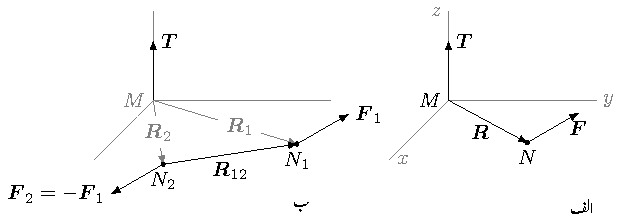
\includegraphics{figInductanceTorqueDefined}
\caption{قوت کا معیار اثر۔}
\label{شکل_امالہ_قوت_کا_معیار_اثر_تعریف}
\end{figure}

یکساں میدان میں پورے دور پر صفر قوت پایا جاتا ہے البتہ دور پر \اصطلاح{قوت گردشہ}\فرہنگ{قوت گردشہ}\حاشیہب{torque}\فرہنگ{torque} یعنی \اصطلاح{قوت کا معیار اثر}\فرہنگ{قوت!معیار اثر}\فرہنگ{معیار اثر!قوت}\حاشیہب{moment of force}\فرہنگ{force!moment of}\فرہنگ{moment!of force} عموماً صفر نہیں ہوتا۔قوت کا معیار اثر حاصل کرنے کی خاطر قوت اور قوت گردشہ کے \اصطلاح{محور} یعنی \اصطلاح{چُول}\فرہنگ{چُول}\حاشیہب{pivot}\فرہنگ{pivot} کا جاننا ضروری ہے۔شکل \حوالہ{شکل_امالہ_قوت_کا_معیار_اثر_تعریف}-الف میں نقطہ \عددیء{N} پر قوت \عددیء{\kvec{F}} عمل کر رہا ہے۔ہم نقطہ \عددیء{M} کو محور چنتے ہیں۔ نقطہ \عددیء{M} سے \عددیء{N} تک سمتی فاصلہ \عددیء{\kvec{R}} قوت کا \اصطلاح{بازو}\فرہنگ{قوت!کا بازو}\فرہنگ{بازو!قوت}\حاشیہب{moment arm}\فرہنگ{moment!arm}  کہلاتا ہے۔قوت کا معیار اثر \عددیء{\kvec{T}}
\begin{align}
\kvec{T}=\kvec{R} \times \kvec{F}
\end{align}
کے برابر ہے۔قوت گردشہ کی قیمت، قوت کے بازو کی لمبائی ضرب قوت کی قیمت ضرب ان دو کے مابین زاویے کے سائن کے برابر ہے جبکہ اس کی سمت دونوں کے عمودی ہے جسے صلیبی ضرب سے حاصل کیا جا سکتا ہے۔

شکل \حوالہ{شکل_امالہ_قوت_کا_معیار_اثر_تعریف}-ب میں  پختہ شکل کے جسم پر دو مختلف نقطوں پر برابر مگر الٹ سمت کے قوت لاگو کئے گئے ہیں۔چونکہ اس جسم پر کل قوت صفر کے برابر ہے لہٰذا یہ کسی بھی سمت میں سیدھی حرکت نہیں کرے گی۔محور \عددیء{M} پر ان قوت گردشہ کا مجموعہ
\begin{align*}
\kvec{T}&=\kvec{R}_1 \times \kvec{F}_1+\kvec{R}_2 \times \kvec{F}_2\\
&=(\kvec{R}_1-\kvec{R}_2) \times \kvec{F}_1\\
&=\kvec{R}_{12} \times \kvec{F}_1
\end{align*}
ہو گا جہاں دوسرے قدم پر  \عددیء{\kvec{F}_2=-\kvec{F}_1} پر کیا گیا ہے۔اس مساوات میں قوتوں کے محور کا \عددیء{\kvec{R}_{12}} پر کوئی اثر نہیں ہے لہٰذا کل قوت صفر ہونے کی صورت میں قوت گردشہ کی قیمت محور پر منحصر نہیں ہے۔اسی عمل کو زیادہ قوتوں پر بھی لاگو کیا جا سکتا ہے۔

چونکہ قوت گردشہ کی قیمت محور پر منحصر نہیں ہے لہٰذا ہم محور اس مقام پر چن سکتے ہیں جس پر قوت گردشہ کا حصول زیادہ آسان ہو۔ہم سطحی قوتوں کی صورت میں ایسا محور عموماً قوتوں کے ہم سطحی ، جسم  کے دھرے پر پایا جاتا ہے۔

\begin{figure}
\centering
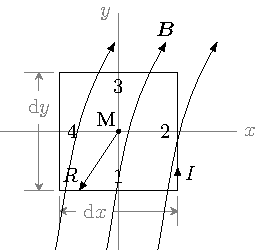
\includegraphics{figInductanceTorqueOnSmallLoop}
\caption{مقناطیسی میدان میں برقی رو گزارتے تفرقی بند دائرے پر قوت گردشہ۔}
\label{شکل_امالہ-تفرقی_دائرے_پر_مروڑ}
\end{figure}

آئیں شکل \حوالہ{شکل_امالہ-تفرقی_دائرے_پر_مروڑ} میں دئے  برقی رو گزارتے تار پر غیر یکساں مقناطیسی میدان \عددیء{\kvec{B}=B_x\ax+B_y \ay+B_z \az} میں قوت گردشہ حاصل کریں۔تصور کریں کہ تار چول \عددیء{M} پر صرف گھوم سکتا ہے۔ اس تار کے اطراف \عددیء{\dif x} اور \عددیء{\dif y} ہیں جبکہ اس میں برقی رو \عددیء{I} کی سمت تیر کے نشان سے ظاہر کی گئی ہے۔اس چھوٹے رقبے کے وسط \عددیء{M} پر مقناطیسی میدان
\begin{align}
\kvec{B}_0=B_{x0}\ax+B_{y0}\ay+B_{z0}\az
\end{align}
کے برابر ہے۔ یوں وسط سے \عددیء{-\tfrac{\dif y}{2}} جانب نقطہ \عددیء{1} پر مقناطیسی میدان ٹیلر تسلسل\فرہنگ{ٹیلر تسلسل}\فرہنگ{Taylor series} سے
\begin{align*}
\kvec{B}_1&=\kvec{B}_0 -\frac{\partial \kvec{B}}{\partial y}\frac{\dif y}{2}+\cdots
\end{align*}
لکھا جا سکتا ہے جہاں تمام تفرق نقطہ \عددیء{M} پر حاصل کئے جاتے ہیں۔صرف ایک درجی تفرق رکھتے ہوئے یوں
\begin{align*}
\kvec{B}_1&=\left(B_{x0}-\frac{\partial B_{x}}{\partial y} \frac{\dif y}{2}\right)\ax+\left(B_{y0}-\frac{\partial B_{y}}{\partial y} \frac{\dif y}{2}\right)\ay+\left(B_{z0}-\frac{\partial B_{z}}{\partial y} \frac{\dif y}{2}\right)\az
\end{align*}
حاصل ہوتا ہے۔یوں راہ کے اس طرف کی  تفرقی لمبائی پر تفرقی قوت
\begin{align*}
\dif \kvec{F}_1=I \dif x \ax \times \kvec{B}_1
\end{align*}
یا
\begin{align*}
\dif \kvec{F}_1&=I \dif x \ax \times \left[\left(B_{x0}-\frac{\partial B_{x}}{\partial y} \frac{\dif y}{2}\right)\ax+\left(B_{y0}-\frac{\partial B_{y}}{\partial y} \frac{\dif y}{2}\right)\ay \right. \\
& \quad \quad\quad \quad\quad \quad\quad \quad\quad \quad\quad \quad\quad\quad \quad \left. +\left(B_{z0}-\frac{\partial B_{z}}{\partial y} \frac{\dif y}{2}\right)\az \right]\\
&=I \dif x \left[\left(B_{y0}-\frac{\partial B_{y}}{\partial y} \frac{\dif y}{2}\right)\az-\left(B_{z0}-\frac{\partial B_{z}}{\partial y} \frac{\dif y}{2}\right)\ay \right]
\end{align*}
ہو گی۔اس قوت کا بازو مرکز سے اس طرف کے درمیانے نقطے تک ہو گا یعنی \عددیء{\kvec{R}_1=-\tfrac{\dif y}{2}\ay} لہٰذا اس قوت کا معیار اثر
\begin{align*}
\dif \kvec{T}_1&=\kvec{R}_1 \times \dif \kvec{F}_1\\
&=-\frac{\dif y}{2}\ay \times I \dif x \left[\left(B_{y0}-\frac{\partial B_{y}}{\partial y} \frac{\dif y}{2}\right)\az-\left(B_{z0}-\frac{\partial B_{z}}{\partial y} \frac{\dif y}{2}\right)\ay \right]\\
&=- \frac{I}{2}\left(B_{y0}-\frac{\partial B_{y}}{\partial y} \frac{\dif y}{2}\right)\dif x \dif y \ax
\end{align*}
ہو گا۔

اسی طرح وسط سے \عددیء{+\tfrac{\dif y}{2}} جانب نقطہ \عددیء{3} پر مقناطیسی میدان مکلارن تسلسل سے
\begin{align*}
\kvec{B}_3&=\kvec{B}_0 +\frac{\partial \kvec{B}}{\partial y}\frac{\dif y}{2}+\cdots
\end{align*}
لکھا جا سکتا ہے جہاں تمام تفرق نقطہ \عددیء{M} پر حاصل کئے جاتے ہیں۔صرف ایک درجی تفرق رکھتے ہوئے یوں
\begin{align*}
\kvec{B}_3&=\left(B_{x0}+\frac{\partial B_{x}}{\partial y} \frac{\dif y}{2}\right)\ax+\left(B_{y0}+\frac{\partial B_{y}}{\partial y} \frac{\dif y}{2}\right)\ay+\left(B_{z0}+\frac{\partial B_{z}}{\partial y} \frac{\dif y}{2}\right)\az
\end{align*}
حاصل ہوتا ہے۔یوں راہ کے اس طرف کی  تفرقی لمبائی پر تفرقی قوت
\begin{align*}
\dif \kvec{F}_3=-I \dif x \ax \times \kvec{B}_3
\end{align*}
یا
\begin{align*}
\dif \kvec{F}_3&=-I \dif x \ax \times \left[\left(B_{x0}+\frac{\partial B_{x}}{\partial y} \frac{\dif y}{2}\right)\ax+\left(B_{y0}+\frac{\partial B_{y}}{\partial y} \frac{\dif y}{2}\right)\ay \right. \\
&\quad \quad \quad \quad\quad \quad \quad \quad\quad \quad \quad \quad\quad \quad \quad \quad \left.+\left(B_{z0}+\frac{\partial B_{z}}{\partial y} \frac{\dif y}{2}\right)\az\right]\\
&=I \dif x \left[-\left(B_{y0}+\frac{\partial B_{y}}{\partial y} \frac{\dif y}{2}\right)\az+\left(B_{z0}+\frac{\partial B_{z}}{\partial y} \frac{\dif y}{2}\right)\ay \right]
\end{align*}
ہو گی۔اس قوت کا بازو مبدا سے اس طرف کے درمیان تک  یعنی \عددیء{\kvec{R}_3=\tfrac{\dif y}{2}\ay} ہے لہٰذا اس قوت کا معیار اثر
\begin{align*}
\dif \kvec{T}_3&=\kvec{R}_3 \times \dif \kvec{F}_3\\
&=\frac{\dif y}{2}\ay \times I \dif x \left[-\left(B_{y0}+\frac{\partial B_{y}}{\partial y} \frac{\dif y}{2}\right)\az+\left(B_{z0}+\frac{\partial B_{z}}{\partial y} \frac{\dif y}{2}\right)\ay \right]\\
&=-\frac{I}{2}\left(B_{y0}+\frac{\partial B_{y}}{\partial y} \frac{\dif y}{2}\right)\dif x \dif y\ax
\end{align*}
ہو گا۔ 

ان دو قوتوں کے معیار اثر کا مجموعہ
\begin{align*}
\dif \kvec{T}_1+\dif \kvec{T}_3=-IB_{y0}\dif x \dif y\ax
\end{align*}
کے برابر ہے۔بالکل اسی طرح تیسرے اور چھوتے اطراف کے قوتوں کے معیار اثر کا مجموعہ
\begin{align*}
\dif \kvec{T}_2+\dif \kvec{T}_4=IB_{x0}\dif x \dif y\ay
\end{align*}
حاصل ہوتا ہے۔یوں تمام اطراف کے قوتوں کے معیار اثر کا مجموعہ
\begin{align*}
\dif \kvec{T}=I \dif x \dif y \left(B_{x0}\ay-B_{y0}\ax \right)
\end{align*}
حاصل ہوتا ہے۔قوسین میں بند حصے کو صلیبی ضرب کی صورت میں لکھا جا سکتا ہے۔یوں
\begin{align*}
\dif \kvec{T}=I \dif x \dif y \left(\az \times \kvec{B}_0 \right)
\end{align*}
یا
\begin{align}\label{مساوات_امالہ_تفرقی_مروڑ_عمومی}
\dif \kvec{T}=I \dif \kvec{S} \times \kvec{B}
\end{align}
حاصل ہوتا ہے جہاں بند راہ سمتی رقبے \عددیء{\dif \kvec{S}} کو گھیرتی ہے۔مندرجہ بالا مساوات میں کثافت مقناطیسی بہاو \عددیء{\kvec{B}} لکھتے ہوئے زیر نوشت نہیں لکھا گیا۔

بند دائرے میں برقی رو ضرب چھوٹے سمتی رقبے  کا حاصل ضرب \اصطلاح{تفرقی مقناطیسی جفت قطب کے معیار اثر}\فرہنگ{معیار اثر!تفرقی مقناطیسی جفت قطب}\فرہنگ{جفت قطب!معیار اثر}\حاشیہب{differential magnetic dipole moment}\فرہنگ{moment!magnetic dipole} \عددیء{\dif \kvec{m}} کی تعریف ہے جس کی اکائی \عددیء{\si{\ampere \meter \squared}} ہے۔یوں
\begin{align}\label{مساوات-امالہ_مقناطیسی_جفت_قطب_معیار_اثر}
\dif \kvec{m}=I \dif \kvec{S}
\end{align}
اور
\begin{align}\label{مساوات_امالہ_تفرقی_مروڑ}
\dif \kvec{T} =\dif \kvec{m} \times \kvec{B}
\end{align}
لکھے جا سکتے ہیں۔

مساوات \حوالہ{مساوات_امالہ_تفرقی_مروڑ_عمومی}، مساوات \حوالہ{مساوات-امالہ_مقناطیسی_جفت_قطب_معیار_اثر} اور مساوات \حوالہ{مساوات_امالہ_تفرقی_مروڑ} عمومی مساوات ہیں جن میں چھوٹا رقبہ \عددیء{\dif \kvec{S}} مربع کے علاوہ کسی بھی شکل کا ہو سکتا ہے اور اس کی سمت کچھ بھی ہو سکتی ہے۔

غیر یکساں مقناطیسی میدان کی صورت میں تار پر کل قوت صفر نہیں ہو گی۔

\begin{figure}
\centering
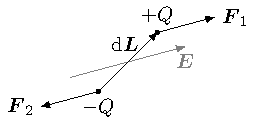
\includegraphics{figInductanceTorqueOnElectricDipole}
\caption{برقی جفت قطب پر برقی میدان میں قوت گردشہ۔}
\label{شکل_امالہ_برقی_جفت_قطب_مروڑ}
\end{figure}

شکل \حوالہ{شکل_امالہ_برقی_جفت_قطب_مروڑ} میں برقی میدان میں برقی جفت قطب دکھایا گیا ہے ۔مثبت بار پر قوت \عددیء{\kvec{F}_1=Q \kvec{E}} اور منفی بار پر قوت   \عددیء{\kvec{F}_2=-Q\kvec{E}} ہے۔ آپ دیکھ سکتے ہیں کہ اس جفت قطب پر  تفرقی قوت گردشہ
\begin{align*}
\dif \kvec{T}&=\dif \kvec{L} \times Q \kvec{E}\\
&=\dif \kvec{p} \times \kvec{E}
\end{align*}
کے برابر ہے جہاں \عددیء{\dif \kvec{p}=Q \dif \kvec{L}} برقی جفت قطب ہے۔قوت گردشہ کی سمت صفحہ کے اندر جانب کو ہے۔ آپ نے دیکھا کہ مقناطیسی اور برقی جفت قطب پر قوت گردشہ کے مساوات یکساں ہیں۔بالکل مقناطیسی جفت قطب کی طرح یہاں بھی قوت گردشہ کا تخمینہ لگاتے وقت جفت قطب کے احاطے میں میدان \عددیء{\kvec{E}} کے تبدیلی کو نظر انداز کیا جا سکتا ہے۔

%===============
\ابتدا{مثال}
شکل \حوالہ{شکل_امالہ-تفرقی_دائرے_پر_مروڑ} میں چھوٹے رقبے کو اتنا چھوٹا تصور کریں کہ اس پر مقناطیسی میدان یکساں تصور کرنا ممکن ہو۔ایسی صورت میں تفرقی قوت گردشہ حاصل کریں۔

حل:یکساں میدان کی صورت میں
\begin{align*}
\dif \kvec{F}_1&=I \dif x \ax \times \left(B_{x0} \ax+B_{y0}\ay+B_{z0}\az\right)\\
&=I \dif x \left(B_{y0}\az-B_{z0}\ay \right)
\end{align*}
اور
\begin{align*}
\dif \kvec{T}_1&=-\frac{\dif y}{2}\ay \times I \dif x \left(B_{y0}\az-B_{z0}\ay \right)\\
&=-\frac{I}{2} \dif x \dif y B_{y0}\ax
\end{align*}
حاصل ہوتے ہیں۔اسی طرح
\begin{align*}
\dif \kvec{F}_3&=-I \dif x \ax \times \left(B_{x0} \ax+B_{y0}\ay+B_{z0}\az\right)\\
&=I \dif x \left(-B_{y0}\az+B_{z0}\ay \right)
\end{align*}
اور
\begin{align*}
\dif \kvec{T}_3&=\frac{\dif y}{2}\ay \times I \dif x \left(-B_{y0}\az+B_{z0}\ay \right)\\
&=-\frac{I}{2} \dif x \dif y B_{y0}\ax
\end{align*}
حاصل ہوتے ہیں۔یوں
\begin{align*}
\dif \kvec{T}_1+\dif \kvec{T}_3=-I \dif x \dif y B_{y0}\ax
\end{align*}
حاصل ہوتے ہیں۔اسی طرح
\begin{align*}
\dif \kvec{T}_2+\dif \kvec{T}_4=I\dif x \dif y  B_{x0}\ay
\end{align*}
حاصل ہوتا ہے۔ان نتائج سے کل قوت گردشہ
\begin{align*}
\dif \kvec{T}=I \dif x \dif y  \left(B_{x0}\ay -B_{y0}\ax\right) 
\end{align*}
ہی حاصل ہوتا ہے۔
\انتہا{مثال}
%================

مندرجہ بالا مثال سے ثابت ہوتا ہے کہ غیر یکساں مقناطیسی میدان کی صورت میں قوت گردشہ حاصل کرتے وقت چھوٹے رقبے پر میدان کی تبدیلی کو نظر انداز کیا جا سکتا ہے۔اس مثال سے یہ بھی ظاہر ہے کہ یکساں مقناطیسی میدان میں تار پر کل قوت صفر کے برابر ہوتی ہے۔ اگر مقناطیسی میدان حقیقت میں یکساں ہی ہو تب کسی بھی بڑے رقبے پر بھی قوت گردشہ بالکل اسی مساوات
\begin{align}\label{مساوات_امالہ_یکساں_میدان_مروڑ_بذریعہ_مقناطیسی_جفت_قطب}
\kvec{T}=I \kvec{S} \times \kvec{B}=\kvec{m} \times \kvec{B} \quad \quad \textrm{\RL{یکساں مقناطیسی میدان}}
\end{align}
سے حاصل ہو گا البتہ غیر یکساں میدان کی صورت میں قوت گردشہ کی تعریف استعمال کرتے ہوئے ہی صحیح جواب حاصل ہو گا۔سوال \حوالہ{سوال_امالہ_مستطیل} میں آپ سے غیر یکساں میدان میں قوت گردشہ حاصل کرنے کو کہا گیا ہے جبکہ سوال \حوالہ{سوال_امالہ_مستطیل_بذریعہ_جفت_قطب} میں مندرجہ بالا مساوات استعمال کرنے کو کہا گیا ہے۔

غور کرنے سے معلوم ہوتا ہے کہ برقی رو گزارتے بند دائرے پر قوت گردشہ اس سمت میں دائرے کو گھمانے کی کوشش کرتا ہے جس میں دائرے سے پیدا مقناطیسی میدان اور بیرونی لاگو مقناطیسی میدان کی سمتیں ایک ہی ہوں۔اس حقیقت کو شکل \حوالہ{شکل_امالہ_مروڑ_مقناطیسی_میدان_متوازی} کی مدد سے یاد رکھا جا سکتا ہے جہاں برقی رو گزارتے تار کی جگہ چھوٹا مقناطیس بیرونی میدان میں دکھایا گیا ہے۔چھوٹا مقناطیس اس سمت میں گھومتا ہے جہاں دونوں میدان متوازی ہوں۔
\begin{figure}
\centering
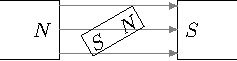
\includegraphics{figInductanceTorqueOnSmallMagnet}
\caption{قوت گردشہ دونوں مقناطیسی میدان کو متوازی بنانے کی کوشش کرتا ہے۔}
\label{شکل_امالہ_مروڑ_مقناطیسی_میدان_متوازی}
\end{figure}
%=================================

\ابتدا{مثال}
محدد \عددی{z} پر لامحدود لمبائی کے تار میں \عددی{I_1} برقی رو \عددی{\az} سمت میں گزر رہی ہے۔اس کے قریب سطح \عددی{z=0} پر تار \عددی{y=a}، \عددی{{-b<x<b}} میں \عددی{-\ax} سمت میں \عددی{I_2} برقی رو گزر رہی ہے۔نقطہ \عددی{(0,a,0)} پر محور تصور کرتے ہوئے لمبی تار کے میدان میں چھوٹی تار پر قوت گردشہ حاصل کریں۔صورت حال شکل \حوالہ{شکل_امالہ_مروڑ_لمبی_اور_چھوٹی_تار} میں دکھائی گئی ہے۔

\begin{figure}
\centering
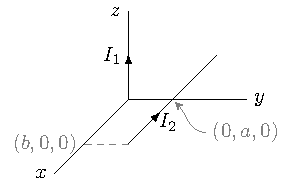
\includegraphics{figInductanceTorqueOnSmallWire}
\caption{چھوٹی تار پر قوت گردشہ کا حصول۔}
\label{شکل_امالہ_مروڑ_لمبی_اور_چھوٹی_تار}
\end{figure}

حل:محدد \عددی{z} پر برقی رو میدان 
\begin{align*}
\kvec{B}=\frac{\mu_0 I_1}{2\pi \rho}\aphi
\end{align*}
پیدا کرتی ہے جسے کارتیسی نظام میں
\begin{align*}
\kvec{B}=\frac{\mu_0 I_1}{2\pi(x^2+y^2)} (-y\ax+x\ay)
\end{align*}
لکھا جا سکتا ہے۔اس میدان کی قیمت اور سمت غیر یکساں ہیں۔کارتیسی میدان میں انتہائی چھوٹی لمبائی کو
\begin{align*}
\dif \kvec{L}=\dif x \ax+\dif y \ay +\dif z \az
\end{align*}
لکھا جاتا ہے۔چھوٹی تار پر \عددی{\dif y=0} اور \عددی{\dif z=0} ہیں لہٰذا \عددی{\dif \kvec{L}=\dif x \ax} لکھتے\حاشیہد{طلباء یہاں عموماً غلطی کرتے ہوئے  \عددی{\dif \kvec{L}=-\dif x \ax} لکھتے ہیں۔یاد رہے کہ تکمل میں ابتدائی اور اختتامی نقطے  دراصل سمت تعین کرتے ہیں۔} ہوئے تار کے انتہائی چھوٹے حصے پر قوت
\begin{align*}
\dif \kvec{F}&=I \dif \kvec{L} \times \kvec{B}\\
&=I_2 \dif x \ax \times \frac{\mu_0 I_1}{2\pi(x^2+y^2)} (-y\ax+x\ay)\\
&=\frac{I_1 I_2 \mu_0 x \dif x \az}{2\pi (x^2+y^2)}
\end{align*}
لکھا جا سکتا ہے۔نقطہ \عددی{(0,a,0)} کو محور تصور کرتے ہوئے \عددی{\kvec{R}=x\ax} لکھا جائے گا۔یوں تار کی انتہائی چھوٹے حصے پر قوت گردشہ
\begin{align*}
\dif \kvec{T}&=\kvec{R} \times \dif \kvec{F}\\
&=x\ax \times \frac{I_1 I_2 \mu_0 x \dif x \az}{2\pi (x^2+y^2)}\\
&=-\frac{I_1 I_2 \mu_0 x^2 \ay}{2\pi (x^2+y^2)} \dif x
\end{align*}
ہو گا۔یوں پورے تار پر کل قوت گردشہ
\begin{align*}
\kvec{T}&=\int_{b}^{-b}-\frac{I_1 I_2 \mu_0 x^2 \ay}{2\pi (x^2+y^2)} \dif x\\
&=\frac{I_1 I_2 \mu_0}{\pi} \left(b-a \tan^{-1} \frac{b}{a}\right)\ay \quad \si{\newton \meter}
\end{align*}
حاصل ہوتا ہے جہاں \عددی{y=a} پر کیا گیا ہے۔
\انتہا{مثال}
%================

\حصہ{فولادی مقناطیسی اشیاء اور مقناطیسی خطے}
شکل \حوالہ{شکل_امالہ_ایٹم_میں_گھومتا_الیکٹران} میں ایٹمی مرکز کے گرد مدار میں گھومتا الیکٹران دکھایا گیا ہے۔حرکت کرتا بار برقی رو پیدا کرتا ہے۔ایسی برقی رو جو مقید الیکٹران کی بنا ہو \اصطلاح{مقید برقی رو}\فرہنگ{برقی رو!مقید}\فرہنگ{مقید!برقی رو}\حاشیہب{bound current}\فرہنگ{current!bound} \عددیء{I_m}  کہلائی جاتی  ہے۔اس الیکٹران کو بند گول دائرے پر مقید برقی رو تصور کیا جا سکتا ہے جو مقناطیسی جفت قطب \عددیء{\kvec{m}} کو جنم دیتی ہے۔الیکٹران منفی ہونے کی وجہ سے   مقید برقی  رو  \عددیء{\kvec{v}} کے الٹ سمت میں ہو گی۔ایٹمی مسائل صرف \اصطلاح{کوانٹم میکانیات}\فرہنگ{کوانٹم میکانیات}\حاشیہب{quantum mechanics}\فرہنگ{quantum mechanics} سے ہی سمجھے جا سکتے ہیں۔یہاں صرف اتنا بتانا ضروری ہے کہ لوہا، نِکل\فرہنگ{نکل}\حاشیہب{nickel}\فرہنگ{nickel} اور کوبالٹ \فرہنگ{کوبالٹ}\حاشیہب{cobolt}\فرہنگ{cobolt} ایسے  عناصر ہیں جن کا  \عددیء{\kvec{m}} قدر زیادہ قیمت رکھتا ہے۔یہ اشیاء \اصطلاح{فولادی مقناطیسی اشیاء}\فرہنگ{فولادی مقناطیسی اشیاء}\حاشیہب{ferromagnetic}\فرہنگ{ferromagnetic} کہلاتے ہیں۔ہم انہیں اشیاء پر غور کرتے ہیں۔

فولادی مقناطیسی اشیاء میں ایٹموں کے باہمی قوتوں کی وجہ سے  قریبی جفت قطب ایک ہی سمت میں رخ کر لیتے ہیں۔ایسے \اصطلاح{ہم صف}\فرہنگ{ہم صف}\حاشیہب{aligned}\فرہنگ{aligned} خطوں میں متعدد ایٹم شامل ہوتے ہیں۔ان خطوں کو \اصطلاح{مقناطیسی خطے}\فرہنگ{مقناطیسی!خطے}\حاشیہب{magnetic domain}\فرہنگ{domain} کہتے ہیں۔مقناطیسی خطے مختلف شکل کے ہو سکتے ہیں اور ان کی جسامت ایک مائیکرو میٹر تا  کئی سنٹی میٹر ممکن ہے۔کسی بھی قدرتی مقناطیسی شہ میں انفرادی مقناطیسی خطے کے مقناطیسی جفت قطب کا معیار اثر انتہائی بڑی مقدار کا ہوتا ہے  البتہ مختلف مقناطیسی خطوں کے جفت قطب کے رخ مختلف سمتوں میں ہوتے ہیں۔اسی وجہ سے پورا حجم از خود کوئی مقناطیسی معیار اثر نہیں رکھتا۔ہاں بیرونی مقناطیسی میدان \عددیء{\kvec{B}_0} لاگو کرنے سے  وہ مقناطیسی خطے جو  \عددیء{\kvec{B}_0} کے  ہی سمت میں رخ کئے ہوں کا حجم بڑھ جاتا ہے جبکہ بقایا مقناطیسی خطوں کا حجم کم ہو جاتا ہے۔یوں اندرونی مقناطیسی میدان بیرونی میدان سے کئی گنا بڑھ جاتا ہے۔بیرونی میدان ہٹا دینے سے تمام مقناطیسی خطے اپنی پرانی صورت اختیار نہیں کر پاتے۔یوں تمام مقناطیسی خطوں کا مجموعی بقایا مقناطیسی معیار اثر رہ جاتا ہے۔یہ حقیقت کہ مقناطیسی اشیاء کے خصوصیات گزشتہ حالات پر منحصر ہے،  \اصطلاح{مقناطیسی چال}\فرہنگ{مقناطیسی!چال}\حاشیہب{hysteresis}\فرہنگ{hysteresis}  کہلاتا ہے۔  
\begin{figure}
\centering
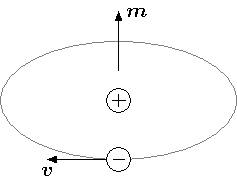
\includegraphics{figInductanceOrbitingElectronInExternalField}
\caption{مدار میں گھومتے الیکٹران کے مقناطیسی جفت قطب کے معیار اثر کو بیرونی میدان کے متوازی دکھایا گیا ہے۔}
\label{شکل_امالہ_ایٹم_میں_گھومتا_الیکٹران}
\end{figure}

\حصہ{مقناطیسیت اور مقناطیسی مستقل}
تصور کریں کہ کسی مادے کے اکائی حجم میں \عددیء{n} مقناطیسی جفت قطب پائے جاتے ہوں۔ اس مادے کے \عددیء{\Delta h} حجم میں \عددیء{n \Delta h} جفت قطب ہوں گے جن کا اجتماعی مقناطیسی معیار اثر ان کا سمتی مجموعہ
\begin{align}
\kvec{m}_{\textrm{کل}}=\sum_{i=1}^{n\Delta h} \kvec{m}_i
\end{align}
ہو گا۔انفرادی \عددیء{\kvec{m}} مختلف قیمت اور سمت کے ہو سکتے ہیں۔اجتماعی مقناطیسی معیار اثر فی اکائی حجم
\begin{align}
\kvec{M}=\lim_{\Delta h \to 0} \frac{1}{\Delta h} \sum_{i=1}^{n \Delta h} \kvec{m}_i
\end{align}
کو \اصطلاح{مقناطیسیت}\فرہنگ{مقناطیسیت}\حاشیہب{magnetization}\فرہنگ{magnetization} پکارا اور  \عددیء{\kvec{M}} سے ظاہر کیا جاتا ہے۔مقناطیسیت کی اکائی  بالکل \عددیء{\kvec{H}} کے اکائی کی طرح ایمپیئر فی میٹر \عددیء{\si{\ampere \per \meter}} ہے۔ مندرجہ بالا مساوات کا صفحہ \حوالہصفحہ{مساوات_موصل_تقطیب_تعریف} پر دئے مساوات \حوالہ{مساوات_موصل_تقطیب_تعریف} کے ساتھ موازنہ کریں جو تقطیب کی تعریف بیان کرتی ہے۔مندرجہ ذیل پڑھتے ہوئے بھی تقطیب پر تبصرے کو ساتھ ساتھ دیکھتے رہیں۔

\begin{figure}
\centering
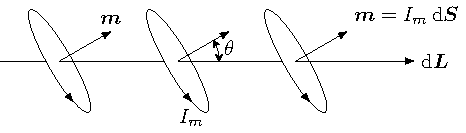
\includegraphics{figInductanceMagnetizationDefined}
\caption{بیرونی مقناطیسی میدان جفت قطب کو صف بستہ کئے ہوئے ہے جس سے بند راہ سے گھیرے گئے سطح میں مقید برقی رو سے اضافہ پایا جاتا ہے۔}
\label{شکل_امالہ_مقناطیسیت_تعریف}
\end{figure}

شکل \حوالہ{شکل_امالہ_مقناطیسیت_تعریف} میں بند راہ کا کچھ حصہ \عددیء{\dif \kvec{L}} دکھایا گیا ہے جس پر مقناطیسی جفت قطب دکھائے گئے ہیں۔چھوٹے رقبے \عددیء{\dif \kvec{S}} کے گرد گھومتی مقید برقی رو \عددیء{I_m} مقناطیسی معیار اثر \عددیء{\kvec{m}=I_m \dif \kvec{S}} کو جنم دیتی ہے۔بیرونی مقناطیسی میدان لاگو کرنے سے جفت قطب ہم صف ہو کر \عددیء{\dif \kvec{L}} کے ساتھ \عددیء{\theta} کا زاویہ بناتے ہیں۔یوں چھوٹے حجم \عددیء{\dif S \cos \theta \dif L} یعنی \عددیء{\dif \kvec{S} \cdot \dif \kvec{L}} میں جفت قطب کی کل تعداد \عددیء{n \dif \kvec{S} \cdot \dif \kvec{L}} ہو گی۔آئیں دیکھتے ہیں کہ بند راہ سے گھیری سطح سے گزرتی برقی رو میں بیرونی میدان لاگو کرنے سے کیا تبدیلی رو نما ہوتی ہے۔اگر بند راہ پر \عددیء{\aL} جانب چلا جائے تو گھیری گئی سطح بائیں ہاتھ کو ہے۔ بیرونی میدان کے غیر موجودگی میں تمام جفت قطب بلا ترتیب پائے جاتے۔بیرونی میدان \عددیء{\kvec{B}} لاگو کرنے کی صورت میں تمام کے تمام \عددیء{n \dif \kvec{S} \cdot \dif \kvec{L}} جفت قطب ہم صف ہو جاتے ہیں جس کی وجہ سے  گھیرے سطح سے کل مقید گزرتی برقی رو بڑھ جاتی ہے۔ہر انفرادی جفت قطب گھیری گئی سطح سے گزرتی برقی رو میں \عددیء{I_m} کا اضافہ کرتا ہے لہٰذا تمام ہم صف جفت قطب مل کر
\begin{align}
\dif I_m=n I_m \dif \kvec{S} \cdot \dif \kvec{L}=\kvec{M} \cdot \dif \kvec{L}
\end{align}
اضافہ پیدا کرتے ہیں۔پورے بند راہ کے گرد چلتے ہوئے یوں کل اضافہ
\begin{align}\label{مساوات_امالہ_مقید_برقی_رو_اور_مقناطیسیت}
I_m=\oint \kvec{M} \cdot \dif \kvec{L}
\end{align}
ہو گا۔ 

مندرجہ بالا مساوات ایمپیئر کے دوری قانون کی مساوات کے ساتھ قریبی مشابہت رکھتا ہے۔یوں \عددیء{\kvec{B}} اور \عددیء{\kvec{H}} کے تعلق پر نظر ثانی کرتے ہوئے یوں بیان کیا جا سکتا ہے کہ یہ خلاء کے علاوہ دیگر اشیاء میں بھی کارآمد ہو۔ہمارا موجودہ تبصرہ بیرونی میدان \عددیء{\kvec{B}} میں جفت قطب پر قوت اور قوت گردشہ پر رہا ہے۔آئیں \عددیء{\kvec{B}} کو ہی بنیادی متغیرہ تصور کرتے ہوئے \عددیء{\kvec{H}} کی بہتر تعریف حاصل کریں۔ایسا کرنے کی خاطر ایمپیئر کے دوری قانون کو آزاد برقی رو \عددیء{I} اور مقید برقی رو \عددیء{I_m} کے مجموعے \عددیء{I_{\textrm{کل}}} کی صورت
\begin{align}\label{مساوات_امالہ_کل_برقی_رو_اور_ایمپیئر_قانون}
\oint \frac{\kvec{B}}{\mu_0} \cdot \dif \kvec{L}=I_{\textrm{کل}}
\end{align}
 میں لکھتے ہیں جہاں
\begin{align}
I_{\textrm{کل}}=I+I_m
\end{align}
کے برابر ہے۔مندرجہ بالا تین مساوات سے
\begin{align}\label{مساوات_امالہ_ایمپیئر_دوری_قانون_بہتر_الف}
I=I_{\textrm{کل}}-I_m=\oint \left(\frac{\kvec{B}}{\mu_0}-\kvec{M} \right) \cdot \dif \kvec{L}
\end{align}
حاصل ہوتا ہے۔قوسین میں بند حصے کو \عددیء{\kvec{H}} کی بہتر تعریف لیتے ہیں یعنی
\begin{align}
\kvec{H}=\frac{\kvec{B}}{\mu_0}-\kvec{M}
\end{align}
جسے یوں
\begin{align}\label{مساوات_امالہ_کثافت_بہاو_شدت_اور_مقناطیسیت}
\kvec{B}=\mu_0\left(\kvec{H}+\kvec{M} \right)
\end{align}
بھی لکھا جا سکتا ہے۔چونکہ خلاء میں \عددیء{\kvec{M}} صفر کے برابر ہوتا ہے لہٰذا مندرجہ بالا مساوات سے خلاء میں \عددیء{\kvec{B}=\mu_0 \kvec{H}} ہی حاصل ہوتا ہے۔مساوات \حوالہ{مساوات_امالہ_ایمپیئر_دوری_قانون_بہتر_الف} میں \عددیء{\kvec{H}} کی نئی تعریف پر کرنے سے ایمپیئر کے دوری قانون کو آزاد برقی رو کی صورت
\begin{align}\label{مساوات_امالہ_آزاد_برقی_رو_اور_شدت}
I=\oint \kvec{H} \cdot \dif \kvec{L}
\end{align}
میں بیان کیا جا سکتا ہے۔

مختلف اقسام کے برقی رو کے لئے
\begin{align*}
I_m&=\oint_S \kvec{J}_m \cdot \dif \kvec{S}\\
I_{\textrm{کل}}&=\oint_S \kvec{J}_{\textrm{کل}} \cdot \dif \kvec{S}\\
I&=\oint_S \kvec{J} \cdot \dif \kvec{S}
\end{align*} 
لکھے جا سکتے ہیں جن سے بذریعہ مسئلہ سٹوکس مساوات \حوالہ{مساوات_امالہ_مقید_برقی_رو_اور_مقناطیسیت}، مساوات \حوالہ{مساوات_امالہ_آزاد_برقی_رو_اور_شدت} اور مساوات \حوالہ{مساوات_امالہ_کل_برقی_رو_اور_ایمپیئر_قانون} کے گردش
\begin{align}
\nabla \times \kvec{M}&=\kvec{J}_m \notag\\
\nabla \times \frac{\kvec{B}}{\mu_0}&=\kvec{J}_{\textrm{کل}} \notag\\
\nabla \times \kvec{H}&=\kvec{J} \label{مساوات_امالہ_آزاد_برقی_رو_اور_گردش}
\end{align}
لکھے جا سکتے ہیں۔ ہمیں یہاں سے آگے مساوات \حوالہ{مساوات_امالہ_آزاد_برقی_رو_اور_شدت} اور مساوات \حوالہ{مساوات_امالہ_آزاد_برقی_رو_اور_گردش} سے غرض رہے گا۔یہ دونوں مساوات آزاد برقی رو کے تعلق پیش کرتے ہیں۔

مساوات \حوالہ{مساوات_امالہ_کثافت_بہاو_شدت_اور_مقناطیسیت} کثافت مقناطیسی  بہاو \عددیء{\kvec{B}}، مقناطیسی میدان کی شدت \عددیء{\kvec{H}} اور مقناطیسیت \عددیء{\kvec{M}} کے تعلق کو بیان کرتی ہے۔خطی\فرہنگ{خطی}\حاشیہب{linear}\فرہنگ{linear} اور \اصطلاح{غیر سمتی خاصیت}\فرہنگ{غیر سمتی خاصیت}\حاشیہب{isotropic}\فرہنگ{isotropic} کے اشیاء  میں مقناطیسیت اور میدان کے شدت کا خطی تعلق
\begin{align}\label{مساوات_امالہ_خطی_ہم_سمتی_اشیاء_تعلق}
\kvec{M}=\chi_m \kvec{H}
\end{align}
پایا جاتا ہے  جہاں \عددیء{\chi_m} کو \اصطلاح{مقناطیسی اثر پذیری}\فرہنگ{مقناطیسی!اثر پذیری}\حاشیہب{magnetic susceptibility}\فرہنگ{magnetic!susceptibility} کہا جاتا ہے۔یوں
\begin{align*}
\kvec{B}&=\mu_0\left(\kvec{H}+\chi_m \kvec{H} \right)\\
&=\mu_0 (1+\chi_m)\kvec{H}
\end{align*}
لکھا جا سکتا ہے۔قوسین میں بند حصے کو \اصطلاح{جزوی مقناطیسی مستقل}\فرہنگ{مقناطیسی!جزوی مستقل}\حاشیہب{relative magnetic constant, relative permeability}\فرہنگ{magnetic!relative constant}\فرہنگ{relative permeability} پکارا اور \عددیء{\mu_R} سے ظاہر کیا جاتا ہے یعنی
\begin{align}
\mu_R=1+\chi_m
\end{align}
یوں
\begin{align*}
\kvec{B}=\mu_0 \mu_R \kvec{H}
\end{align*}
یا
\begin{align}
\kvec{B}=\mu \kvec{H}
\end{align}
حاصل ہوتا ہے جہاں \عددیء{\mu}
\begin{align}
\mu=\mu_0 \mu_R
\end{align}
\اصطلاح{مقناطیسی مستقل}\فرہنگ{مقناطیسی!مستقل}\حاشیہب{magnetic constant, permeability}\فرہنگ{permeability}\فرہنگ{magnetic!constant} پکارا جاتا ہے۔جزوی مقناطیسی مستقل \عددیء{\mu_R} کے استعمال سے بایوٹ سیوارٹ کا قانون اور ایمپیئر کے دوری قانون کو خلاء کے علاوہ ان تمام اشیاء میں بھی استعمال کیا جا سکتا ہے جو خطی اور غیر سمتی خاصیت رکھتے ہوں۔ایسے اشیاء مساوات \حوالہ{مساوات_امالہ_خطی_ہم_سمتی_اشیاء_تعلق} پر پورا اترتے ہیں۔

فولادی مقناطیسی اشیاء کے \عددیء{\mu_R} کی قیمت \عددیء{10} تا \عددیء{\num{100000}} پائی جاتی ہے۔

\اصطلاح{سمتی خاصیت}\فرہنگ{سمتی خاصیت}\حاشیہب{anisotropic}\فرہنگ{anisotropic} کے اشیاء میں \عددیء{\kvec{H}} کا ہر کارتیسی جزو \عددیء{\kvec{B}} کے ہر کارتیسی جزو پر اثر انداز ہوتا ہے لہٰذا ان کا تعلق تناوی\فرہنگ{تناوی}\فرہنگ{tensor} شکل
\begin{gather}
\begin{aligned}\label{مساوت_امالہ_تناوی-مساوات}
B_x&=\mu_{xx} H_x +\mu_{xy} H_y+\mu_{xz} H_z\\
B_y&=\mu_{yx} H_x +\mu_{yy} H_y+\mu_{yz} H_z\\
B_z&=\mu_{zx} H_x +\mu_{zy} H_y+\mu_{zz} H_z
\end{aligned}
\end{gather}
میں لکھا جا سکتا ہے۔یہ مساوات صفحہ \حوالہصفحہ{مساوت_کپیسٹر_تناوی-مساوات} پر دئے مساوات \حوالہ{مساوت_کپیسٹر_تناوی-مساوات} کی طرح ہے۔یوں سمتی خاصیت کے اشیاء میں \عددیء{\kvec{B}=\mu \kvec{H}} کے تعلق میں \عددیء{\mu} تناوی مستقل ہے۔مساوات \عددیء{\kvec{B}=\mu_0(\kvec{H}+\kvec{M})} اب بھی درست ہے اگرچہ \عددیء{\kvec{B}}، \عددیء{\kvec{H}} اور \عددیء{\kvec{M}} عموماً غیر متوازی ہوں گے۔

مقناطیسی اثر پذیری کی بات کرتے ہوئے خطی تعلق تصور کیا گیا ہے۔حقیقت میں ایسا خطی تعلق صرف غیر مقناطیسی اشیاء میں ہی پایا جاتا ہے۔

\حصہ{مقناطیسی سرحدی شرائط}\فرہنگ{سرحدی شرائط!مقناطیسی میدان}\فرہنگ{مقناطیسی میدان!سرحدی شرائط}\فرہنگ{boundary conditions!magnetic field}\فرہنگ{magnetic field!boundary conditions}

ہم موصل اور ذو برق کے سرحدی شرائط دیکھ چکے ہیں۔انہیں دیکھتے ہوئے آگے پڑھیں۔بالکل انہیں کی طرح شکل \حوالہ{شکل_امالہ_مقناطیسی_سرحدی_شرائط} کی مدد سے مقناطیسی سرحدی شرائط حاصل کرتے ہیں جہاں دو مقناطیسی اشیاء کا سرحد دکھایا گیا ہے جن کے مقناطیسی مستقل \عددیء{\mu_1} اور \عددیء{\mu_2} ہیں۔ سرحد پر چھوٹے نلکی ڈبے کی لمبائی کم سے کم کرتے ہوئے گاوس کے قانون
\begin{align*}
\oint_S \kvec{B} \cdot \dif \kvec{S}=0
\end{align*}
کے اطلاق سے
\begin{align*}
B_{n1}\Delta S-B_{n2} \Delta S=0
\end{align*}
یعنی
\begin{align}\label{مساوات_امالہ_عمودی_مقناطیسی_میدان_بے_جوڑ_ہے}
B_{n2}=B_{n1}
\end{align}
یا
\begin{align}
H_{n2}=\frac{\mu_1}{\mu_2} H_{n1}
\end{align}
حاصل ہوتے ہیں۔یوں عمودی \عددیء{\kvec{B}} سرحد پر بلا جوڑ\فرہنگ{بلا جوڑ}\فرہنگ{continuous} ہے جبکہ عمودی \عددیء{\kvec{H}} سرحد پر \عددیء{\frac{\mu_1}{\mu_2}} کی شرح سے جوڑ دار\فرہنگ{جوڑ دار}\فرہنگ{discontinuous} ہے۔مندرجہ بالا دو مساوات کو یوں
\begin{align}
\aN  \cdot \left(\kvec{B}_2-\kvec{B}_1 \right)&=0\\
\aN \cdot \left(\kvec{H}_2-\frac{\mu_1}{\mu_2} \kvec{H}_1 \right)&=0
\end{align}
بھی لکھا جا سکتا ہے۔
 \begin{figure}
\centering
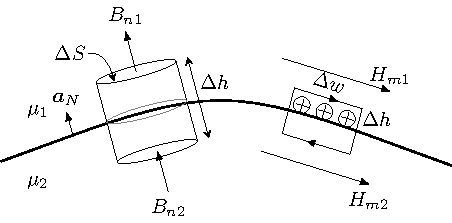
\includegraphics{figInductanceMagneticBoundaryConditions}
\caption{مقناطیسی سرحدی شرائط۔}
\label{شکل_امالہ_مقناطیسی_سرحدی_شرائط}
\end{figure}

سرحد پر عمودی \عددیء{\kvec{M}} کا تعلق سرحد پر عمودی \عددیء{\kvec{H}} کے تعلق سے حاصل ہوتا ہے۔خطی خاصیت کے مقناطیسی اشیاء کے لئے یوں
\begin{align}
M_{n2}=\frac{\chi_{m2}}{\chi_{m1}}\frac{\mu_1}{\mu_2}M_{n1}
\end{align}
لکھا جا سکتا ہے۔

سرحد پر انتہائی کم موٹائی کے خطے میں کثافت برقی رو \عددیء{K} تصور کرتے ہوئے کثافت کے عمودی \عددیء{\Delta L} چوڑائی پر برقی رو \عددیء{I_{\Delta L}=K \Delta L} لکھی جا سکتی ہے۔یوں سرحد پر متوازی اجزاء کا شرط شکل میں مستطیل راہ پر ایمپیئر کے دوری قانون
\begin{align*}
\oint \kvec{H} \cdot \dif \kvec{L}=I
\end{align*}
کے اطلاق سے
\begin{align*}
H_{m1} \Delta w -H_{m2}\Delta w=K_\perp \Delta w
\end{align*}
یعنی
\begin{align}
H_{m1} -H_{m2}=K_\perp
\end{align}
 حاصل ہوتا ہے جہاں \عددیء{K_{\perp}} سے مراد \عددیء{K} کا وہ حصہ ہے جو \عددیء{H_{m1}} اور \عددیء{H_{m2}} کے عمودی ہے۔سمتی ضرب کے استعمال سے مندرجہ بالا مساوات کو
\begin{align}
\aN \times \left(\kvec{H}_1-\kvec{H}_2 \right)  =\kvec{K}_{\perp}
\end{align}
لکھا جا سکتا ہے جہاں \عددیء{\aN} سرحد پر عمودی اکائی سمتیہ  ہے۔ سرحد کے متوازی \عددیء{\kvec{B}} کے لئے یوں
\begin{align}
\frac{B_{m1}}{\mu_1}-\frac{B_{m2}}{\mu_2}=K_\perp
\end{align}
یا
\begin{align}
\aN \times \left(\frac{B_{m1}}{\mu_1}-\frac{B_{m2}}{\mu_2}\right)=\kvec{K}_\perp
\end{align}
لکھا جا سکتا ہے۔اسی طرح خطی خاصیت کے اشیاء کے لئے سرحد کے متوازی \عددیء{\kvec{M}} کے لئے
\begin{align}
M_{m2}=\frac{\chi_{m2}}{\chi_{m1}} M_{m1}-\chi_{m2} K_\perp
\end{align}
لکھا جا سکتا ہے۔سرحد پر صفر کثافت برقی رو کی صورت میں مندرجہ بالا تین مساوات سادہ صورت اختیار کر لیتے ہیں۔دونوں اشیاء غیر موصل ہونے کی صورت میں سرحد پر کثافت برقی رو صفر ہی ہوتی ہے۔
%======================
\ابتدا{مثال}
مساوات \عددی{3x-2y+5z<1} خطہ-1 جبکہ مساوات \عددی{3x-2y+5z>1} خطہ-2 کو ظاہر کرتی ہے۔ ان خطوں کے جزوی مقناطیسی مستقل \عددی{\mu_{R1}=2.5} اور \عددی{\mu_{R2}=5} ہیں ۔خطہ-1 میں \عددی{\kvec{H}_1=30\ax+20\ay-40\az} ہے۔سرحد کے عمودی، خطہ-1 سے خطہ-2 کی جانب  اکائی سمتیہ \عددی{\aN} حاصل کریں۔پہلے خطے  میں سرحد کے عمودی اور متوازی میدان کے اجزاء حاصل کریں۔اسی طرح دوسرے خطے میں سرحد کے عمودی اور متوازی میدان حاصل کریں۔سرحد کے عمود کے ساتھ دونوں خطوں میں میدان کیا زاویہ بناتا ہے۔

حل:سرحدی مساوات کی ڈھلوان سے اکائی سمتیہ حاصل ہو گی۔چونکہ ڈھلوان کی سمت بڑھتے جانب ہوتی ہے لہٰذا اس کی سمت خطہ-1 سے خطہ-2 کی جانب ہو گی۔
\begin{align*}
\aN&=\frac{\nabla (3x-2y+5z)}{\abs{\nabla (3x-2y+5z)}}\\
&=\frac{3\ax-2\ay+5\az}{\sqrt{38}}\\
&=0.487\ax-0.324\ay+0.811\az
\end{align*} 

میدان کا عمودی جزو
\begin{align*}
\kvec{H}_{n1}&=(\kvec{H}_1 \cdot \aN) \aN\\
&=-24.33(0.487\ax-0.324\ay+0.811\az)\\
&=-11.84\ax+7.89\ay-19.74\az
\end{align*}
ہے جسے میدان سے منفی کرنے سے متوازی جزو حاصل ہو گا۔
\begin{align*}
\kvec{H}_{m1}&=\kvec{H}_1-\kvec{H}_{n1}\\
&=(30\ax+20\ay-40\az)-(-11.84\ax+7.89\ay-19.74\az)\\
&=41.84\ax+12.11\ay-20.26\az
\end{align*}
چونکہ سرحد پر مقناطیسی میدان بے جوڑ ہوتا ہے لہٰذا سرحد  کے دونوں اطراف پر متوازی میدان برابر ہوں گے۔
\begin{align*}
\kvec{H}_{m2}=\kvec{H}_{m1}=41.84\ax+12.11\ay-20.26\az
\end{align*}
سرحدی شرائط سے 
\begin{align*}
\kvec{H}_{n2}=\frac{\mu_{R1}}{\mu_{R2}} \kvec{H}_{n1}&=\frac{2}{5}(-11.84\ax+7.89\ay-19.74\az)\\
&=-5.92\ax+3.95\ay-9.87\az
\end{align*}
لکھا جا سکتا ہے۔یوں دوسرے خطے میں میدان
\begin{align*}
\kvec{H}_2=\kvec{H}_{m2}+\kvec{H}_{n2}=35.92\ax+16.05\ay-30.13\az
\end{align*}
ہے۔پہلے خطے میں
\begin{align*}
\cos \theta_1&=\frac{\abs{\kvec{H}_{n1}}}{\abs{\kvec{H}_1}}=0.452
\end{align*}
سے
\begin{align*}
\theta_1=63.1^{\circ}
\end{align*}
حاصل ہوتا ہے جبکہ دوسرے خطے میں اسی طرح
\begin{align*}
\theta_2=\cos^{-1} \frac{\abs{\kvec{H}_{n2}}}{\abs{\kvec{H}_2}}=75.8^{\circ}
\end{align*}
حاصل ہوتا ہے۔
\انتہا{مثال}
%======================
\حصہ{مقناطیسی دور}
یک سمتی برقی ادوار حل کرنے سے آپ بخوبی آگاہ ہوں گے۔کئی مقناطیسی مسائل بالکل انہیں کی طرح حل ہوتے ہیں۔برقی مشین مثلاً موٹر اور ٹرانسفارمر کے کارکردگی پر غور کرتے وقت انہیں مقناطیسی ادوار سمجھا جاتا ہے۔میری کتاب "برقی آلات" میں اس ترکیب پر پورا باب ہے اور پوری کتاب میں اسی ترکیب کو استعمال کرتے ہوئے مختلف برقی مشین پر غور کیا گیا ہے۔ آئیں اس ترکیب کو دیکھیں۔

سب سے پہلے ان برقی اور مقناطیسی مساوات کو پاس پاس لکھتے ہیں جن کی مدد سے مقناطیسی ادوار کا تصور پیدا ہوتا ہے۔برقی دباو اور برقی میدان کی شدت کا تعلق
\begin{align}
\kvec{E}=-\nabla V
\end{align}
ہے۔غیر سمتی مقناطیسی دباو اور مقناطیسی میدان کی شدت کے تعلق
\begin{align}
\kvec{H}=-\nabla V_m
\end{align}
سے بھی آپ بخوبی واقف ہیں۔منبع برقی دباو کو محرک برقی دباو پکارا جاتا ہے۔اسی مشابہت کی بنا پر غیر مقناطیسی  دباو کو محرک مقناطیسی دباو پکارا جائے گا۔متحرک مقناطیسی دباو کی اکائی ایمپیئر ہے۔حقیقت میں عموماً متعدد چکر کے لچھے کو بطور متحرک مقناطیسی دباو استعمال کیا جاتا ہے اور  یوں اس کی اکائی ایمپیئر-چکر\فرہنگ{ایمپیئر چکر}\حاشیہب{ampere-turns}\فرہنگ{ampere-turns} لی جاتی ہے۔یاد رہے کہ غیر سمتی مقناطیسی دباو صرف اس خطے میں معنی رکھتا ہے جہاں برقی رو موجود نہ ہو۔

دو نقطوں کے درمیان برقی دباو کے فرق کو
\begin{align}
V_{AB}=-\int_B^A \kvec{E} \cdot \dif \kvec{L}
\end{align}
لکھا جاتا ہے۔بالکل اسی طرح دو نقطوں کے درمیان مقناطیسی دباو کے فرق کو
\begin{align}
V_{mAB}=-\int_B^A \kvec{H} \cdot \dif \kvec{L}
\end{align}
لکھا جاتا ہے۔صفحہ \حوالہصفحہ{مساوات_مقناطیسی_غیر_سمتی_دباو_خطہ} پر مساوات \حوالہ{مساوات_مقناطیسی_غیر_سمتی_دباو_خطہ} میں بتلایا گیا کہ غیر سمتی مقناطیسی دباو کے حصول کے دوران مندرجہ بالا تکمل میں \عددیء{\phi=\pi} پر سے نہیں گزرا جائے گا۔اس حقیقت کا خیال رکھنا ضروری ہے۔ 

برقی ادوار میں اوہم  کے قانون کی نقطہ شکل
\begin{align}
\kvec{J}=\sigma \kvec{E}
\end{align}
سے کون خبردار نہیں ہے۔یہ مساوات کثافت برقی رو اور برقی میدان کے شدت کا تعلق بیان کرتی ہے۔مقناطیسی ادوار میں اس کا مقابل
\begin{align}
\kvec{B}=\mu \kvec{H}
\end{align}
ہے جو کثافت مقناطیسی بہاو اور مقناطیسی میدان کے شدت کا تعلق پیش کرتی ہے۔

کل برقی رو بذریعہ سطحی تکمل
\begin{align}
I=\int_S \kvec{J} \cdot \dif \kvec{S}
\end{align}
حاصل ہوتی ہے۔کل مقناطیسی بہاو  بھی ایسے ہی تکمل سے حاصل ہو گا لہٰذا
\begin{align}
\Phi=\int_S \kvec{B} \cdot \dif \kvec{S}
\end{align}
لکھا جائے گا۔یوں برقی ادوار میں \عددیء{I} اور مقناطیسی ادوار میں \عددیء{\Phi} اہمیت کے حامل ہیں۔

برقی ادوار میں برقی دباو اور برقی رو کی شرح کو برقی مزاحمت پکارا اور \عددیء{R} سے ظاہر کیا جاتا ہے یعنی
\begin{align}
V=I R
\end{align}
 ہم بالکل اسی طرح متحرک مقناطیسی دباو اور مقناطیسی بہاو کی شرح کو ہچکچاہٹ کا نام دیتے ہیں جسے \عددیء{\Re} سے ظاہر کیا جائے گا لہٰذا مقناطیس ادوار کے لئے
\begin{align}
V_m=\Phi \Re
\end{align}
لکھا جا سکتا ہے۔ہچکچاہٹ کی اکائی ایمپیئر-چکر فی ویبر \عددیء{(\si{\ampere \cdot t \per \weber})} ہے۔

خطی اور غیر سمتی خاصیت کے  یکساں مادہ جس کی موصلیت \عددیء{\sigma} ہو سے بنایا گیا برقی مزاحمت
\begin{align}
R=\frac{d}{\sigma S}
\end{align}
کے برابر ہے جہاں مزاحمت کی لمبائی \عددیء{d} اور اس کا رقبہ عمودی تراش پورے لمبائی پر یکساں \عددیء{S} کے برابر ہے۔اگر خطی اور غیر سمتی خاصیت کے یکساں مادہ سے ہچکچاہٹ بنایا جائے تو اس کی قیمت
\begin{align}
\Re=\frac{d}{\mu S}
\end{align}
ہو گی جہاں ہچکچاہٹ کی لمبائی \عددیء{d} اور اس کا رقبہ عمودی تراش پورے لمبائی پر یکساں \عددیء{S} کے برابر ہے۔حقیقت میں ہوا کے علاوہ ایسا کوئی مادہ نہیں پایا جاتا جس سے اٹل قیمت کی ہچکچاہٹ بنائی جا سکے۔

%===================
\ابتدا{مثال}
ایک سلاخ جس کی لمبائی \عددیء{\SI{15}{\centi\meter}} اور رداس \عددیء{\SI{1}{\milli\meter}} ہے کی موصلیت \عددیء{\SI{1200}{\siemens\per\meter}} ہے پر \عددیء{\SI{220}{\volt}} برقی دباو لاگو کی جاتی ہے۔سلاخ کی مزاحمت اور اس میں برقی رو حاصل کریں۔سلاخ میں کثافت برقی رو بھی حاصل کریں۔

حل:مزاحمت
\begin{align*}
R=\frac{d}{\sigma A}=\frac{0.15}{7 \times 10^4 \times \pi \times 0.001^2}=\SI{39.8}{\ohm}
\end{align*}
اور برقی رو
\begin{align*}
I=\frac{V}{R}=\frac{220}{39.8}=\SI{5.5}{\ampere}
\end{align*}
اور یوں کثافت برقی رو ہو گا
\begin{align*}
J=\frac{I}{A}=\frac{5.5}{\pi\times 0.001^2}=\SI{1.75}{\mega \ampere \per \meter \squared}
\end{align*}
\انتہا{مثال}
%===========
\ابتدا{مثال}
ایک سلاخ جس کی لمبائی \عددیء{\SI{15}{\centi\meter}} اور رداس \عددیء{\SI{2}{\centi\meter}} ہے کا جزو مقناطیسی مستقل \عددیء{1000} ہے۔اس پر \عددیء{100} چکر کا لچھا جس میں \عددیء{\SI{0.5}{\ampere}} برقی رو ہو مقناطیسی دباو لاگو کرتا ہے۔سلاخ کی ہچکچاہٹ اور اس میں مقناطیسی بہاو حاصل کریں۔سلاخ میں کثافت مقناطیسی بہاو بھی حاصل کریں۔

حل:ہچکچاہٹ
\begin{align*}
\Re=\frac{d}{\mu_R \mu_0 A}=\frac{0.15}{1000\times 4 \times \pi \times 10^{-7} \times \pi \times  0.02^2}=\SI{94988}{\ampere \cdot t \per \weber}
\end{align*}
اور مقناطیسی بہاو
\begin{align*}
\Phi=\frac{V_m}{\Re}=\frac{100 \times 0.5}{94988}=\SI{0.53}{\milli \weber}
\end{align*}
اور یوں کثافت مقناطیسی بہاو ہو گی
\begin{align*}
B=\frac{\Phi}{A}=\frac{0.00053}{\pi \times 0.02^2}=\SI{0.42}{\tesla}
\end{align*}
\انتہا{مثال}
%==================
\حصہ{مقناطیسی مخفی توانائی}
ساکن برقی میدان پر غور کے دوران ہم نے نقطہ بار پر قوت کے تجرباتی نتائج سے کولمب کا قانون اخذ کیا۔اس قانون کو استعمال کرتے ہوئے  مختلف نقطہ بار  کو لامحدود فاصلے سے مختلف اختتامی مقامات پر رکھنے کی خاطر کل درکار توانائی حاصل کی گئی۔یہی ساکن برقی میدان کی مخفی توانائی تھی۔اس مخفی توانائی کی عمومی مساوات
\begin{align}
W_{\textrm{برقی}}=\frac{1}{2}\int_h \kvec{D} \cdot \kvec{E} \dif h
\end{align}
ہے جہاں \عددیء{\kvec{D}} اور \عددیء{\kvec{E}} کا تعلق راست تناسب تصور کیا گیا ہے۔

یہاں خیال آتا ہے کہ مقناطیسی میدان کی مخفی توانائی بھی اسی طرز پر حاصل کی جا سکتی ہے جیسے برقی میدان کی مخفی توانائی حاصل کی گئی تھی، یعنی، ایک برقی رو گزارتے تار کے قریب دوسرے برقی رو گزارتے تار کو قریب لاتے ہوئے درکار توانائی معلوم کر کے۔حقیقت میں معاملہ اتنا سادہ نہیں ہے۔جیسے کہ اگلے باب میں بتلایا جائے گا، مقناطیسی میدان میں حرکت کرتے حصے میں برقی دباو پیدا ہوتا ہے جس میں معاملہ خاصہ تبدیل ہو جاتا ہے۔

مقناطیسی میدان کی مخفی توانائی\فرہنگ{مخفی توانائی!مقناطیسی میدان}\فرہنگ{potential energy!magnetic field} اگلے باب میں \اصطلاح{پوئنٹنگ سمتیہ}\فرہنگ{پوئنٹنگ سمتیہ}\حاشیہب{Poynting vector}\فرہنگ{Poynting vector} سے حاصل کی جائے گی۔یہاں مقناطیسی مخفی توانائی کی مساوات صرف پیش کرتے ہیں
\begin{align}\label{مساوات_امالہ_مخفی_توانائی_الف}
W_{\textrm{مقناطیسی}}=\frac{1}{2}\int_h \kvec{B} \cdot \kvec{H} \dif h
\end{align} 
جو شکل سے برقی مخفی توانائی کے مساوات کے قریبی مشابہت رکھتا ہے۔اس میں \عددیء{\kvec{B}=\mu \kvec{H}} پر کرنے سے
\begin{align}\label{مساوات_امالہ_مخفی_توانائی_ب}
W_{\textrm{مقناطیسی}}=\frac{1}{2}\int_h \mu H^2 \dif h
\end{align}
اور
\begin{align}\label{مساوات_امالہ_مخفی_توانائی_پ}
W_{\textrm{مقناطیسی}}=\frac{1}{2}\int_h  \frac{B^2}{\mu} \dif h
\end{align}
بھی حاصل ہوتے ہیں۔

برقی مخفی توانائی کی طرح یہاں بھی یہ بتلانا کہ مخفی توانائی درحقیقت کہاں پر ہے نا ممکن ثابت ہوتا ہے البتہ حساب و کتاب آسان بنانے کی خاطر ہم فرض کر سکتے ہیں کہ یہ توانائی پورے حجم میں بطور کثافت توانائی \عددیء{\tfrac{1}{2}\kvec{B}\cdot\kvec{H}} پائی جاتی ہے جسے جاول فی مربع میٹر \عددیء{\si{\joule \per \meter^3}} میں ناپا جائے گا۔


%====================
\حصہ{خود امالہ اور مشترکہ امالہ}
برقی ادوار میں مزاحمت، برق گیر\حاشیہب{capacitor} (کپیسٹر) اور \اصطلاح{امالہ گیر}\فرہنگ{امالہ گیر}\حاشیہب{inductor}\فرہنگ{inductor} کردار ادا کرتے ہیں۔مزاحمت اور برق گیر (کپیسٹر) پر ہم بات کر چکے ہیں۔برقی دباو اور برقی رو کی شرح کو مزاحمت کہا گیا۔ ہم نے دیکھا کہ مزاحمت کے قیمت کا دارومدار مزاحمت کے لمبائی، رقبہ عمودی تراش اور موصلیت پر ہے۔اسی طرح دو چادروں میں سے کسی ایک پر بار کی حتمی قیمت اور ان چادروں  کے درمیان برقی دباو کی شرح کو برقی گنجائش (کپیسٹنس) کہا گیا۔ہم نے دیکھا کہ برقی گنجائش کے قیمت کا دارومدار برق گیر (کپیسٹر) کے چادروں کے رقبے، ان چادروں کے درمیان فاصلے اور چادروں کے درمیان مادے کی برقی مستقل پر ہے۔یوں مزاحمت اور برق گیر (کپیسٹر) کے قیمت ان کے شکل، جسامت اور مادے کے مستقل پر ہے۔اس حصے میں ہم امالہ گیر کی \اصطلاح{امالیت} \عددیء{L} پر غور کریں گے جس کی اکائی \اصطلاح{ہینری}\فرہنگ{ہینری}\حاشیہب{Henry}\فرہنگ{Henry} \عددیء{\si{\henry}} ہے۔\اصطلاح{امالہ گیر}\حاشیہب{inductor} اور اس کی \اصطلاح{امالیت}\حاشیہب{inductance} دونوں کے لئے ہم \اصطلاح{امالہ}\فرہنگ{امالہ} کا لفظ استعمال کریں گے۔نیچے کئی مساوات میں امالہ اور فاصلہ دونوں کے لئے ایک ہی علامت یعنی \عددیء{L} استعمال کیا گیا ہے۔امید کی جاتی ہے کہ متن سے ان کا فرق کرنا ممکن ہو گا۔ہم دیکھیں گے کہ اس کے قیمت کا دارومدار امالہ گیر کی شکل، جسامت اور مقناطیسی مستقل پر ہے۔ 

امالہ سمجھنے کی خاطر \اصطلاح{ارتباط بہاو}\فرہنگ{ارتباط بہاو}\حاشیہب{flux linkage}\فرہنگ{flux linkage} کا ذکر ضروری ہے۔تصور کریں کہ \عددیء{N} چکر لا لچھا جس میں \عددیء{I} برقی رو گزر رہا ہے کل \عددیء{\Phi} مقناطیسی بہاو پیدا کرتا ہے۔تصور کریں کہ \عددیء{\Phi} ان تمام \عددیء{N} چکر سے گزرتی ہے۔یوں تمام کا تمام مقناطیسی بہاو ہر چکر سے گزرتی ہے۔یوں پہلے چکر سے \عددیء{\Phi} بہاو گزرتی ہے، دوسرے چکر سے بھی \عددیء{\Phi} بہاو گزرتی ہے اور اسی طرح بقایا ہر چکر سے بھی اتنی ہی بہاو گزرتی ہے۔ارتباط بہاو سے مراد \عددیء{N \Phi} ہے یعنی تمام چکر سے گزرتی بہاو کا مجموعہ۔

ارتباط بہاو اور برقی رو کی شرح کو امالہ کہا جاتا ہے۔اگر ارتباط بہاو اسی برقی رو سے پیدا ہو تب ان کی شرح کو \اصطلاح{خود امالہ}\فرہنگ{خود امالہ}\فرہنگ{امالہ!خود}\حاشیہب{self inductance}\فرہنگ{self inductance} کہتے ہیں جسے عموماً چھوٹا کر کے صرف \اصطلاح{امالہ}\فرہنگ{امالہ} پکارا جاتا ہے۔اس کے برعکس اگر برقی رو ایک تار میں ہو اور ارتباط بہاو دوسری تار کی ہو تب ان کے شرح کو \اصطلاح{مشترکہ امالہ}\فرہنگ{امالہ!مشترکہ}\فرہنگ{مشترکہ امالہ}\حاشیہب{mutual inductance}\فرہنگ{mutual inductance} کہتے ہیں۔اس حصے میں خود امالہ پر ہی غور کیا جائے گا۔اگلے حصے میں مشترکہ امالہ پر غور کیا جائے گا۔ 
\begin{align}
L=\frac{N \Phi}{I}
\end{align}
اس مساوات میں تصور کیا گیا ہے کہ پورا مقناطیسی بہاو تمام چکر سے گزرتی ہے۔امالہ کی یہ تعریف صفر خطی مقناطیسی اشیاء کے لئے معنی رکھتی ہے۔خطی مقناطیسی اشیاء سے مراد ایسے مقناطیسی اشیاء ہیں جن میں مقناطیسی بہاو اور برقی رو راست تناسب کا تعلق رکھتے ہیں۔فولادی مقناطیسی اشیاء میں مقناطیسی چال کی بنا پر امالہ کی کوئی ایک تعریف تمام موقعوں کے لئے کارآمد ثابت نہیں ہوتا۔ہم خطی مقناطیسی اشیاء تک ہی بحث کو محدود رکھیں گے۔

آئیں ہم محوری تار\فرہنگ{ہم محوری تار!امالہ}\فرہنگ{coaxial!inductance} کے اکائی لمبائی کی امالہ حاصل کریں۔صفحہ \حوالہصفحہ{مساوات_مقناطیسی_ہم_محوری_تاروں_کے_درمیان_شدت} پر مساوات \حوالہ{مساوات_مقناطیسی_ہم_محوری_تاروں_کے_درمیان_شدت}
\begin{align*}
H_{\phi}=\frac{I}{2\pi \rho} \quad \quad (\rho_1 < \rho <\rho_2)
\end{align*}
 ہم محوری تار میں تاروں کے درمیانی خطے میں مقناطیسی شدت دیتا ہے جسے استعمال کرتے ہوئے اس خطے میں \عددیء{z_0} لمبائی پر کل مقناطیسی بہاو
\begin{align*}
\Phi&=\int_S B_{\phi} \dif S\\
&=\int_0^{z_0} \int_{\rho_1}^{\rho_2}\frac{\mu I \dif \rho \dif z}{2\pi \rho}\\
&=\frac{\mu  I z_0}{2\pi} \ln \frac{\rho_2}{\rho_1}
\end{align*}
حاصل کیا جا سکتا ہے۔یہ مقناطیسی بہاو دونوں تاروں کے درمیانے خطے میں  اندرونی تار کے گرد گھومتی ہے لہٰذا تکمل میں کسی بھی زاویہ پر \عددیء{z_0} لمبی \عددیء{\rho_1} تا \عددیء{\rho_2} رداسی سطح لی جا سکتی ہے۔یوں اکائی لمبائی پر ہم محوری تار  کی امالہ
\begin{align}\label{مساوات_امالہ_ہم_محوری_کم_تعددی_امالہ}
L=\frac{\mu  I }{2\pi} \ln \frac{\rho_2}{\rho_1}
\end{align}
ہو گی۔یہاں \عددیء{N=1} یعنی ایک ہی چکر ہے اور تمام کا تمام مقناطیسی بہاو پورے برقی رو کے گرد چکر کاٹتی ہے۔
\begin{figure}
\centering
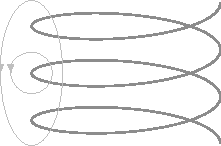
\includegraphics{figInductanceMultiTurnInductance}
\caption{متعدد چکر کے لچھے میں ہر چکر سے گزرتی مقناطیسی بہاو مختلف ہو سکتی ہے۔}
\label{شکل_امالہ_متعدد_چکر}
\end{figure}

اب تصور کریں کہ پیچدار لچھے کی امالہ درکار ہو جسے شکل \حوالہ{شکل_امالہ_متعدد_چکر} میں دکھایا گیا ہے۔ایسے لچھے  کے پہلے چکر کا پورا بہاو پہلے چکر سے گزرتی ہے البتہ اس کا کچھ ہی حصہ دوسرے یا تیسرے چکر سے گزرتی ہے۔یہی کچھ بقایا چکر کے بارے میں بھی کہا جا سکتا ہے۔ایسی صورت میں لچھے کی ارتباط بہاو حاصل کرنے کی خاطر ہر چکر سے گزرتی انفرادی بہاو لیتے ہوئے تمام کا مجموعہ حاصل کیا جائے گا یعنی
\begin{align*}
\textrm{\RL{ارتباط بہاو}}= \Phi_1+\Phi_2+\cdots +\Phi_N=\sum_{i=1}^{N} \Phi_i
\end{align*}
آئیں اب امالہ کی عمومی مساوات حاصل کریں۔ 

کسی بھی بند راہ پر یک سمتی برقی رو \عددیء{I} گزرنے سے کثافت مقناطیسی بہاو \عددیء{\kvec{B}}
\begin{align*}
\kvec{B}=\nabla \times \kvec{A}
\end{align*}
 پیدا ہوتی  ہے جہاں \عددیء{\kvec{A}} سمتی مقناطیسی دباو ہے جسے
\begin{align*}
\kvec{A}=\frac{\mu_0 I}{4\pi}\oint \frac{\dif \kvec{L}}{R}
\end{align*}
سے حاصل کیا جا سکتا ہے۔ایسی بند راہ سطح \عددیء{S} کو گھیرتی ہے جس میں سے گزرتی کل مقناطیسی بہاو  \عددیء{\Phi} کو تکمل
\begin{align*}
\Phi=\int_S \kvec{B} \cdot \dif \kvec{S}
\end{align*}
سے حاصل کیا جا سکتا ہے۔اس تکمل میں \عددیء{\kvec{B}} پر کرنے سے
\begin{align*}
\Phi=\int_S \left(\nabla \times \kvec{A}  \right) \cdot \dif \kvec{S}
\end{align*}   
حاصل ہوتا ہے۔مسئلہ بایوٹ سیوارٹ کی مدد سے اسے
\begin{align*}
\Phi=\oint \kvec{A} \cdot \dif \kvec{L}
\end{align*}
لکھا جا سکتا ہے جہاں بند تکمل سطح کے سرحد یعنی برقی رو گزارتے بند راہ پر حاصل کیا جائے گا۔اس مساوات میں \عددیء{\kvec{A}} پر کرنے سے
\begin{align*}
\Phi=\frac{\mu_0 I}{4\pi}\oint\left(\oint \frac{\dif \kvec{L}}{R} \right) \cdot \dif \kvec{L}
\end{align*}
حاصل ہوتا ہے۔یوں امالہ کی عمومی مساوات 
\begin{align}
L=\frac{\mu_0 }{4\pi}\oint\left(\oint \frac{\dif \kvec{L}}{R} \right) \cdot \dif \kvec{L}
\end{align}
حاصل ہوتی ہے۔یہاں تکمل کے اندر \عددیء{L} فاصلے کو ظاہر کرتی ہے جبکہ مساوات کے بائیں ہاتھ یہی علامت امالہ کو ظاہر کرتی ہے۔

امالہ کی مساوات سے ظاہر ہے کہ امالہ کی قیمت کا دارومدار صرف اور صرف تار یا لچھے کی شکل و جسامت اور مقناطیسی مستقل پر منحصر ہے۔

امالہ کی مساوات حاصل کرنے کی خاطر سطحی تکمل لیا گیا۔ایک چکر کے بند راہ جس سطح کو گھیرتی ہے، اس کی شکل ذہن میں آسانی سے بن جاتی ہے البتہ پیچدار لچھا جس سطح کو گھیرتا ہے اس کی شکل ذہن میں ذرا مشکل\حاشیہد{آپ لچھے کے محور پر سلاخ تصور کرتے ہوئے اس کے گرد گول گھومتی اور اوپر جاتی سطح تصور کر سکتے ہیں۔} سے بنتی ہے۔سطحی تکمل لیتے وقت ایسی تمام ممکنہ سطح استعمال کی جا سکتی ہیں جن کا سرحد پیچدار لچھے کی تار ہو۔

برقی رو گزارتے تار کی رداس صفر کرنے سے بایوٹ سیوارٹ کے قانون کے تحت لامحدود کثافت مقناطیسی بہاو حاصل ہو گی جس سے لامحدود توانائی اور لامحدود امالہ حاصل ہوتا ہے۔حقیقت میں قابل استعمال جوابات حاصل کرنے کی خاطر تار کے رداس  چھوٹا ضرور لیکن صفر کبھی تصور نہیں کیا جاتا۔

کسی بھی برقی رو گزارتے تار کے اندر بھی زاویائی مقناطیسی بہاو پایا جاتا ہے۔تار کے محور کے قریب  گھومتی اندرونی بہاو کم برقی رو کو گھیرتی ہے جبکہ محور سے دور زاویائی اندرونی بہاو زیادہ برقی رو گھیرتی ہے۔جیسا آپ اگلے بابوں میں پڑھیں گے، زیادہ تعدد پر تار کے بیرونی سطح کے قریب زیادہ برقی رو گزرتی ہے لہٰذا زیادہ تعدد پر تار کی اندرونی امالہ کا کردار قابل نظرانداز ہوتا ہے البتہ کم تعدد پر اس کا حساب رکھنا ضروری ہوتا ہے۔

%===============
\ابتدا{مثال}
محوری تار میں اندرونی تار کا رداس \عددی{\rho_1} جبکہ بیرونی تار کا رداس \عددی{\rho_2} ہے۔ان تاروں کے درمیان خطہ \عددی{0<\phi<90^{\circ}} میں \عددی{\mu_R=2} مقناطیسی مستقل کا ذو برق بھرا گیا ہے جبکہ بقایا خطہ خلاء پر مشتمل ہے۔تاروں کے درمیان خطے میں مقناطیسی بہاو حاصل کرتے ہوئے فی میٹر تار کی امالہ حاصل کریں۔

حل:ایمپیئر کا قانون استعمال کرتے ہوئے تاروں کے درمیان میدان حاصل کرتے ہیں۔اندرونی تار میں برقی رو \عددی{I} تصور کرتے ہوئے تاروں کے درمیان میدان \عددی{\aphi} سمت میں پیدا ہو گا۔ذو برق اور خلاء کے سطح پر میدان عمودی ہے۔مساوات \حوالہ{مساوات_امالہ_عمودی_مقناطیسی_میدان_بے_جوڑ_ہے}
\begin{align*}
B_{n1}=B_{n2}
\end{align*}
 کے تحت دو ذو برق کے ملاپ پر مقناطیسی میدان کا عمودی جزو بے جوڑ ہوتا ہے۔یوں ہم محوری تار میں ذو برق کی سرحد پر \عددی{B_{\phi}} بے جوڑ ہو گا۔یوں رداس \عددی{\rho} پر خلاء اور ذو برق میں یکساں \عددی{B_{\phi}} پایا جائے گا۔اس طرح خلاء میں \عددی{H_{\phi}=\tfrac{B_{\phi}}{\mu_0}} ہو گا جبکہ ذو برق میں \عددی{H_{\phi}=\tfrac{B_{\phi}}{\mu_R \mu_0}} ہو گا۔اس حقیقت کو استعمال کرتے ہوئے ایمپیئر کے قانون کو یوں لکھا جا سکتا ہے
\begin{align*}
\oint \kvec{H} \cdot \dif \kvec{L}=\frac{B_{\phi}}{\mu_R \mu_0} \frac{\pi}{2} \rho+\frac{B_{\phi}}{\mu_0} \frac{3\pi}{2} \rho=I
\end{align*} 
جس سے 
\begin{align*}
\kvec{B}=\frac{2\mu_0 I}{\pi \rho \left(\frac{1}{\mu_R}+3\right)} \aphi
\end{align*}
حاصل ہوتا ہے۔یوں فی میٹر لمبائی لیتے ہوئے دونوں تاروں کے درمیان مقناطیسی بہاو
\begin{align*}
\Phi&=\int_0^{1} \int_{\rho_1}^{\rho_2} \frac{2\mu_0 I}{\pi \rho \left(\frac{1}{\mu_R}+3\right)} \dif \rho \dif z\\
&=\frac{2\mu_0 I}{\pi  \left(\frac{1}{\mu_R}+3\right)} \ln \frac{\rho_2}{\rho_1}
\end{align*}
ہو گا جس سے امالہ
\begin{align*}
L=\frac{\Phi}{I}=\frac{2\mu_0}{\pi  \left(\frac{1}{\mu_R}+3\right)} \ln \frac{\rho_2}{\rho_1}
\end{align*}
حاصل ہوتی ہے۔

\انتہا{مثال}
%=================
\ابتدا{مثال}
لا محدود لمبائی کے تار کی اندرونی امالہ حاصل کریں۔

حل:رداس \عددیء{\rho_1} کے تار کو \عددیء{z} محدد پر تصور کرتے ہیں۔تار میں کثافت برقی رو یکساں تصور کرتے ہوئے \عددیء{J=\tfrac{I}{\pi \rho_1^2}} حاصل ہوتا ہے۔رداس \عددیء{\rho} پر گول دائرہ \عددیء{\tfrac{I\rho^2}{\rho_1^2}} برقی رو گھیرتا ہے لہٰذا ایمپیئر کے دوری قانون کے تحت اس دائرے پر زاویائی شدت \عددیء{H_{\phi}=\tfrac{I\rho}{2\pi\rho_1^2}} ہو گی۔رداس \عددیء{\rho} پر \عددیء{\dif \rho} چوڑائی اور \عددیء{z_0} لمبائی کی مستطیل سطح سے 
\begin{align*}
\dif \Phi=B_{\phi} z_0 \dif \rho=\mu H_{\phi} z_0 \dif \rho
\end{align*}
بہاو گزرے گی۔اگر تار کو متعدد باریک متوازی تاروں کا مجموعہ تصور کیا جائے تو مندرجہ بالا تفرقی بہاو صفر \عددیء{\rho} کے اندر تاروں کو گھیرتی ہے جو ایک چکر کا صرف 
\عددیء{\tfrac{\rho^2}{\rho_1^2}} حصہ ہیں لہٰذا یہ تفرقی بہاو صرف  
\begin{align*}
\textrm{\RL{تفرقی ارتباط بہاو}}=\frac{\rho^2}{\rho_1^2} \dif \Phi=\frac{\rho^2}{\rho_1^2}\mu H_{\phi} z_0 \dif \rho=\frac{\mu I z_0}{2\pi \rho_1^4}\rho^3\dif \rho
\end{align*}
دیتی ہے۔اگر تفرقی بہاو تمام فرضی باریک تاروں کو گھیرتی تب یہ ایک چکر شمار ہوتا۔یوں تکمل سے اندرونی ارتباط بہاو
\begin{align*}
\textrm{\RL{ارتباط بہاو}}=\int_0^{\rho_1}\frac{\mu I z_0}{2\pi \rho_1^4}\rho^3\dif \rho=\frac{\mu I z_0}{8\pi}
\end{align*}
 حاصل ہوتی ہے جس سے اندرونی امالہ
\begin{align*}
L_{\textrm{اندرونی}}=\frac{\mu  z_0}{8\pi}
\end{align*}
یا فی میٹر امالہ
\begin{align}\label{مساوات_امالہ_ہم_محوری_اندرونی_تار}
L_{\textrm{\RL{اندرونی فی میٹر}}}=\frac{\mu }{8\pi}
\end{align}

حاصل ہوتی ہے۔
\انتہا{مثال}
%==========
\ابتدا{مشق}\شناخت{مثال_امالہ_ہم_محوری_بیرونی_تار_کی_اندرونی_امالہ}
صفحہ \حوالہصفحہ{شکل_مقناطیسی_ہم_محوری_تار} میں ہم محوری تار\فرہنگ{ہم محوری تار!امالہ}\فرہنگ{coaxial!inductance} دکھائی گئی ہے۔بیرونی تار کی اندرونی امالہ حاصل کریں۔

جوابات:تار کی لمبائی \عددیء{z_0} لیتے ہوئے
\begin{align*}
I_{\textrm{گھیرا}}&=\left(\frac{\rho_3^2-\rho^2}{\rho_3^2-\rho_2^2}\right)I\\
H_{\phi}&=\frac{I}{2\pi \rho} \left(\frac{\rho_3^2-\rho^2}{\rho_3^2-\rho_2^2} \right) \\
\dif \Phi&=\mu H_{\phi} z_0 \dif \rho
\end{align*}
حاصل ہوتا ہے۔یہ تفرقی بہاو ایک چکر کے \عددیء{\frac{\rho_3^2-\rho^2}{\rho_3^2-\rho_2^2}} حصے کے گرد گھومتی ہے لہٰذا تفرقی ارتباط بہاو
\begin{align*}
\textrm{\RL{تفرقی ارتباط بہاو}}=\frac{\mu I z_0}{2\pi \rho} \left(\frac{\rho_3^2-\rho^2}{\rho_3^2-\rho_2^2} \right)^2 \dif \rho
\end{align*}
اور یوں \عددیء{z_0=1} پر کرتے ہوئے فی میٹر امالہ
\begin{align}\label{مساوات_امالہ_ہم_محوری_بیرونی_تار}
L_{\textrm{\RL{بیرونی تار}}}=\frac{\mu}{2\pi \left(\rho_3^2-\rho_2^2\right)^2}\left(\rho_3^4 \ln \frac{\rho_3}{\rho_2}-\frac{\rho_2^4}{4}-\frac{3\rho_3^4}{4}+\rho_2^2 \rho_3^2\right)
\end{align}
حاصل ہوتی ہے۔
\انتہا{مشق}
%=========

مساوات \حوالہ{مساوات_امالہ_ہم_محوری_اندرونی_تار} ہی ہم محوری تار کے اندرونی تار کی امالہ دیتا ہے۔یوں کم تعدد پر مساوات \حوالہ{مساوات_امالہ_ہم_محوری_کم_تعددی_امالہ}، مساوات \حوالہ{مساوات_امالہ_ہم_محوری_اندرونی_تار} اور مساوات \حوالہ{مساوات_امالہ_ہم_محوری_بیرونی_تار} کا مجموعہ
\begin{align}\label{مساوات_امالہ_ہم_محوری_کم_تعددی_فی_میٹر_کل_امالہ}
L=\frac{\mu  I }{2\pi} \ln \frac{\rho_2}{\rho_1}+\frac{\mu }{8\pi}+\frac{\mu}{2\pi \left(\rho_3^2-\rho_2^2\right)^2}\left(\rho_3^4 \ln \frac{\rho_3}{\rho_2}-\frac{\rho_2^4}{4}-\frac{3\rho_3^4}{4}+\rho_2^2 \rho_3^2\right)
\end{align}
فی میٹر ہم محوری تار کا  کل امالہ ہو گا۔جیسے اگلے بابوں میں بتلایا جائے گا، بلند تعدد پر تار میں کثافت برقی رو یکساں نہیں رہتی جس کی وجہ سے تار کی اندرونی امالہ قابل نظرانداز ہو جاتی ہے۔یوں بلند تعدد پر مساوات \حوالہ{مساوات_امالہ_ہم_محوری_کم_تعددی_امالہ} ہی فی میٹر تار کی امالہ دے گا۔

آپ امالہ کے مخفی توانائی
\begin{align}
W=\frac{L I^2}{2}
\end{align}
سے بخوبی واقف ہیں جہاں مخفی توانائی مساوات \حوالہ{مساوات_امالہ_مخفی_توانائی_الف}، مساوات \حوالہ{مساوات_امالہ_مخفی_توانائی_ب} یا مساوات \حوالہ{مساوات_امالہ_مخفی_توانائی_پ} سے حاصل کی جا سکتی ہے۔انہیں استعمال کرتے ہوئے امالہ یوں بھی حاصل کی جا سکتی ہے۔
\begin{gather}
\begin{aligned}\label{مساوات_امالہ_مخفی_توانائی_ت}
L=\frac{2W}{I^2}&=\frac{1}{I^2}\int_h \kvec{B} \cdot \kvec{H} \dif h\\
&=\frac{1}{I^2}\int_h \mu H^2 \dif h\\
&=\frac{1}{I^2}\int_h \frac{B^2}{\mu} \dif h
\end{aligned}
\end{gather}

آپ سے مندرجہ بالا مساوات استعمال کرتے  ہوئے، سوال \حوالہ{سوال_امالہ_لامحدود_لمبی_تار} میں لامحدود لمبائی کے سیدھی تار کی امالہ اور سوال \حوالہ{سوال_امالہ_ہم-محوری_بیرونی_تار_اندرونی_ امالہ} میں ہم محوری تار کے بیرونی تار کی اندرونی امالہ حاصل کرنے کو کہا گیا ہے۔
%================
\حصہ{مشترکہ امالہ} 
شکل \حوالہ{مساوات_امالہ_مشترکہ_امالہ} میں دو تار دکھائے گئے ہیں۔آئیں پہلی تار میں برقی رو \عددیء{I} سے پیدا مقناطیسی بہاو کا وہ حصہ حاصل کریں جو  دوسرے تار سے گزرتا ہے۔ان معلومات سے دونوں تاروں  کے مابین \اصطلاح{مشترکہ امالہ}\فرہنگ{امالہ!مشترکہ}\فرہنگ{مشترکہ امالہ}\فرہنگ{mutual inductance}\حاشیہب{mutual inductance}\فرہنگ{inductance!mutual} حاصل کیا جائے گا۔
\begin{figure}
\centering
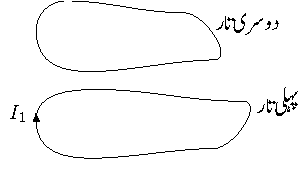
\includegraphics{figInductanceMutualInductance}
\caption{مشترکہ امالہ۔}
\label{مساوات_امالہ_مشترکہ_امالہ}
\end{figure}
خود امالہ حاصل کرنے کے  طرز پر دوسرے تار سے گزرتی بہاو کو 
\begin{align*}
\Phi_{2} =\frac{\mu_0 I_1}{4\pi} \oint \left(\oint \frac{\dif \kvec{L}_1}{R} \right) \cdot \dif \kvec{L}_2
\end{align*}
لکھا جا سکتا ہے جہاں اندرونی تکمل پہلی تار پر ہے اور یہ کسی بھی نقطے پر مقناطیسی میدان دیتا ہے جبکہ دوسری تکمل دوسرے تار پر ہے جس میں سے گزرتی بہاو کا حصول درکار ہے۔مشترکہ امالہ \عددیء{M_{21}} کی تعریف
\begin{align}
M_{21}=\frac{\Phi_2}{I_1}
\end{align}
ہے جس سے
\begin{align}\label{مساوات_امالہ_مشترکہ_الف}
M_{21}=\frac{\mu_0}{4\pi} \oint \left(\oint \frac{\dif \kvec{L}_1}{R} \right) \cdot \dif \kvec{L}_2
\end{align}
حاصل ہوتا ہے۔

اگر دوسری تار میں برقی رو لی جاتی اور پہلی سے گزرتی بہاو حاصل کی جاتی تب
\begin{align}
M_{12}=\frac{\mu_0}{4\pi} \oint \left(\oint \frac{\dif \kvec{L}_2}{R} \right) \cdot \dif \kvec{L}_1
\end{align}
حاصل ہوتا۔مندرجہ بالا دو درجی تکمل میں اندرونی تکمل دوسری راہ پر ہے جبکہ بیرونی تکمل پہلی راہ پر ہے۔تکمل لینے کی ترتیب بدلتے ہوئے اگر پہلا تکمل پہلی راہ پر لیا جائے اور بعد میں دوسری راہ پر تکمل لیا جائے تو تکمل کی قیمت میں کوئی تبدیلی رونما نہیں ہو گی لیکن ایسا کرنے سے ہمیں ہو بہو مساوات \حوالہ{مساوات_امالہ_مشترکہ_الف} ملتا ہے  لہٰذا 
\begin{align}
M_{21}=M_{12}
\end{align}
حاصل ہوتا ہے۔یہ انتہائی اہم نتیجہ ہے جس کے تحت کسی بھی دو لچھوں کے درمیان مشترکہ امالہ دونوں جانب سے برابر حاصل ہوتی ہے۔



%==========================
\newpage
\حصہء{سوالات}
%=====================
\ابتدا{سوال}
میدان \عددی{\kvec{E}=1.5\az \, \si{\volt\per\meter}} میں الیکٹران  حرکت کرتا ہے۔لمحہ \عددی{t=0} پر الیکٹران نقطہ \عددی{(0,0,0)} پر پایا جاتا ہے جبکہ اس کی سمتی رفتار \عددی{\kvec{v}=3\times 10^{5}\ax \, \si{\meter\per\second}} ہے۔الیکٹران کا بار \عددی{\SI{-1.6e-19}{\coulomb}} اور اس کی کمیت \عددی{\SI{3.1e-31}{\kilo\gram}} ہے۔نیوٹن کے قوانین حرکت سے تفرقی مساوات لکھ کر اسے حل کرتے ہوئے لمحہ \عددی{t=\SI{150}{\nano\second}} پر الیکٹران کی سمتی رفتار، مقام اور حرکی توانائی دریافت کریں۔

جوابات:\عددی{\kvec{v}=\num{300000}\ax-\num{116129}\az \, \si{\meter\per\second}}، \عددی{(0.045,0,-3.48)}، \عددی{\SI{1.63e-20}{\joule}}
\انتہا{سوال}
%=====================
\ابتدا{سوال}
مقناطیسی میدان \عددی{\kvec{B}=0.3\ax-0.2\ay-0.4\az \, \si{\tesla}} میں لمحہ \عددی{t=0} پر الیکٹران کی سمتی رفتار \عددی{\kvec{v}=10^6 \az \si{\meter\per\second}} ہے۔الیکٹران پر قوت دریافت کریں۔ایسا برقی میدان حاصل کریں جس کی موجودگی میں مقناطیسی اور برقی میدان مل کر اس الیکٹران پر صفر قوت  پیدا کرتے ہیں۔

جواب:\عددی{\kvec{F}=-32\ax-48\ay \, \si{\femto\newton}}، \عددی{\kvec{E}=-200\ax-300\ay \, \si{\volt\per\meter}}
\انتہا{سوال}
%====================
\ابتدا{سوال}
میدان \عددی{\kvec{B}=2\ax-1\ay+3\az \, \si{\tesla}} اور \عددی{\kvec{E}=3\ax+2\ay-1\az \, \si{\volt\per\meter}} میں بار \عددی{\SI{1.2}{\micro\coulomb}} حرکت کر رہا ہے۔لمحہ \عددی{t=0} پر اس کی رفتار \عددی{\kvec{v}=10\ax-30\ay+20\az \, \si{\kilo\meter\per\second}} ہے۔یہ بار \عددی{\SI{5}{\micro\gram}} کے کمیت پر پایا جاتا ہے۔لمحہ \عددی{t=0} پر بار کی اسراع حاصل کریں۔

جواب:\عددی{\kvec{a}=-16.8\ax+2.4\ay+12\az \, \si{\mega\meter\per\second\squared}}
\انتہا{سوال}
%======================
\ابتدا{سوال}
محدد \عددی{z} پر پڑی لامحدود لمبائی کے تار میں \عددی{5\az \, \si{\ampere}} برقی رو گزر رہی ہے۔اس کے قریب سطح \عددی{x=0} پر موصل تار \عددی{N_1(0,1,0)}، \عددی{N_2(0,4,0)}، \عددی{N_3(0,4,2)} اور \عددی{N_4(0,1,2)} نقطوں کو جوڑ کر مستطیل بناتی ہے جس میں \عددی{N_1} سے \عددی{N_2} جانب \عددی{\SI{2}{\ampere}} برقی رو چکر  لگا رہی ہے۔چکور کے چاروں اطراف پر قوت دریافت کرتے ہوئے پورے چکور پر قوت حاصل کریں۔

جوابات:تار \عددی{N_1(0,1,0)} تا \عددی{N_2(0,4,0)} پر قوت \عددی{2.77\az \, \si{\micro\newton}} ہے۔یہاں سے گھڑی کے الٹ سمت چلتے ہوئے بقایا قوت  \عددی{-1\ay\, \si{\micro\newton}}، \عددی{-2.77\az \, \si{\micro\newton}} اور \عددی{4\ay\, \si{\micro\newton}} ہیں۔یوں مستطیل پر کل قوت \عددی{3\ay\, \si{\micro\newton}} ہے۔
\انتہا{سوال}
%======================
\ابتدا{سوال}
محدد \عددی{z} پر پڑی لامحدود لمبائی کے تار میں \عددی{10\az \, \si{\ampere}} برقی رو گزر رہی ہے۔اس کے قریب نقطہ \عددی{N_1(2,1,3)} سے \عددی{N_2(5,4,7)} تک سیدھی موصل تار میں \عددی{N_1} سے \عددی{N_2} جانب \عددی{\SI{4}{\ampere}} برقی رو گزر رہی ہے۔چھوٹی تار پر قوت حاصل کریں۔

جواب:\عددی{\kvec{F}=-6.74\ax-4.49\ay+8.42\az \, \si{\micro\newton}}
\انتہا{سوال}
%========================
\ابتدا{سوال}
سطح \عددی{x=0} پر مقناطیسی میدان کا \عددی{z} جزو \عددی{B_z=\tfrac{200}{z^2+1} \, \si{\micro \tesla}} پایا جاتا ہے۔اس مقناطیسی جزو سے خطہ \عددی{1<y<3}، \عددی{-\infty <z< \infty} میں کثافت \عددی{\kvec{K}=0.2\ay \si{\ampere\per\meter}} پر قوت حاصل کریں۔

جواب:\عددی{251\ax \, \si{\micro\newton}}
\انتہا{سوال}
%=======================
\ابتدا{سوال}
\عددی{z} محدد پر پڑی لامحدود لمبائی کے تار میں \عددی{\SI{2.2}{\ampere}} برقی رو پائی جاتی ہے۔سطح \عددی{y=0} پر خطہ \عددی{\SI{1}{\milli\meter} < x < \SI{5}{\milli\meter}} پر \عددی{\az} سمت میں کل \عددی{\SI{8}{\ampere}} برقی رو گزر رہی ہے۔اس خطے کی فی میٹر لمبائی پر مقناطیسی قوت حاصل کریں۔محدد \عددی{z} پر پڑی تار پر بھی فی میٹر قوت حاصل کریں۔

جواب:\عددی{-1.4\ax \, \si{\milli\newton}}، \عددی{1.4\ax \, \si{\milli\newton}}
\انتہا{سوال}
%=======================
\ابتدا{سوال}
محدد \عددی{z} پر پڑی لامحدود لمبائی کی تار میں \عددی{I_1} برقی رو \عددی{\az} جانب گزر رہی ہے۔اس کے قریب سطح \عددی{z=0} پر تار \عددی{y=a}، \عددی{-b<x<b} میں \عددی{I_2} برقی رو \عددی{\ax} سمت میں گزر رہی ہے۔نقطہ \عددی{(0,0,0)} کو محور لیتے ہوئے چھوٹی تار پر قوت گردشہ حاصل کریں۔صفحہ \حوالہصفحہ{شکل_امالہ_مروڑ_لمبی_اور_چھوٹی_تار} پر شکل \حوالہ{شکل_امالہ_مروڑ_لمبی_اور_چھوٹی_تار} میں صورت حال دکھایا گیا ہے۔

جواب:\عددی{-\frac{I_1 I_2 \mu_0}{\pi} \left(b-a \tan^{-1} \frac{b}{a}\right)\ay \,\si{\newton \meter}}
\انتہا{سوال}
%=====================
\ابتدا{سوال}\شناخت{سوال_امالہ_مستطیل}
موصل تار نقطہ \عددی{N_1(2,0,0)}، \عددی{N_2(5,0,0)}، \عددی{N_3(5,0,4)} اور \عددی{N_4(2,0,4)} کو جوڑ کر مستطیل بناتی ہے۔مثبت \عددی{y} محدد کی جانب سے دیکھتے ہوئے، اس مستطیل میں \عددی{\SI{6}{\ampere}} برقی رو سمت گھڑی گردش کر رہی ہے۔الف)  یکساں میدان \عددی{\kvec{B}=5\ax \, \si{\tesla}} کی صورت میں \عددی{z} محدد  کو محور لیتے ہوئے مستطیل کے چاروں اطراف پر علیحدہ علیحدہ  قوت گردشہ حاصل کرتے ہوئے کل قوت گردشہ حاصل کریں۔ ب) سطح \عددی{y=0} پر لکیر \عددی{x=3} کو محور لیتے ہوئے اسی یکساں میدان میں دوبارہ قوت گردشہ حاصل کریں۔

جوابات:(الف) اور (ب):مستطیل کے چار حصوں پر قوت گردشہ \عددی{0}، \عددی{600\az \, \si{\newton \meter}}، \عددی{0} اور \عددی{-240\az\, \si{\newton\meter}} ہے۔یوں کل قوت گردشہ \عددی{360\az \, \si{\newton\meter}} حاصل ہوتا ہے۔
\انتہا{سوال}
%======================
\ابتدا{سوال}\شناخت{سوال_امالہ_مستطیل_بذریعہ_جفت_قطب}
سوال \حوالہ{سوال_امالہ_مستطیل} میں میدان یکساں ہے لہٰذا اس میں محور کا قوت گردشہ پر کوئی اثر نہیں ہوتا۔ایسی صورت میں قوت گردشہ صفحہ \حوالہصفحہ{مساوات_امالہ_یکساں_میدان_مروڑ_بذریعہ_مقناطیسی_جفت_قطب} پر دئے  مساوات \حوالہ{مساوات_امالہ_یکساں_میدان_مروڑ_بذریعہ_مقناطیسی_جفت_قطب} کی مدد سے حاصل کی جا سکتی ہے۔ایسا ہی کریں۔

جواب:\عددی{360\az \, \si{\newton\meter}}
\انتہا{سوال}
%================================
\ابتدا{سوال}
سوال \حوالہ{سوال_امالہ_مستطیل} میں یکساں میدان کی جگہ اگر \عددی{z} محدد پر لامحدود لمبائی کے تار میں \عددی{\az} جانب \عددی{\SI{25}{\ampere}} برقی رو میدان پیدا کرے تب محدد کے مبدا \عددی{(0,0,0)} کو محور لیتے ہوئے قوت گردشہ حاصل کریں۔یاد رہے کہ یہ میدان غیر یکساں ہے لہٰذا مساوات  \حوالہ{مساوات_امالہ_یکساں_میدان_مروڑ_بذریعہ_مقناطیسی_جفت_قطب} قابل استعمال نہیں ہے۔

جواب:مستطیل کے چار حصوں پر قوت گردشہ \عددی{-90\ay \, \si{\micro \newton \meter}}، \عددی{-48\ay \, \si{\micro \newton \meter}}، \\
\عددی{90\ay \, \si{\micro \newton \meter}} اور \عددی{120\ay \, \si{\micro \newton \meter}}  ہے جس سے کل قوت گردشہ  \عددی{72\ay \, \si{\micro\newton\meter}} حاصل ہوتا ہے۔
\انتہا{سوال}
%=============================
\ابتدا{سوال}
دو سنٹی میٹر رداس اور پانچ سو چکر کے پیچ دار لچھے میں \عددی{\SI{3}{\ampere}} کی برقی رو گزر رہی ہے۔یہ لچھا \عددی{\SI{1.5}{\tesla}} کے میدان میں پایا جاتا ہے۔میدان اور لچھے کے محور آپس میں عمودی ہیں۔ لچھے پر قوت گردشہ حاصل کریں۔

جواب:\عددی{\SI{2.83}{\newton \meter}}
\انتہا{سوال}
%========================
\ابتدا{سوال}
ایک مادہ  میدان \عددی{\kvec{B}=0.15z\ay \, \si{\tesla}} میں پایا جاتا ہے۔اس مادے کی \عددی{\chi=2.5} ہے۔آپ سے گزارش ہے کہ \عددی{\mu_R}، \عددی{\kvec{H}}، \عددی{\kvec{M}}، \عددی{\kvec{J}} ،\عددی{\kvec{J}_m} اور \عددی{\kvec{J}_T} حاصل کریں۔

جوابات: \عددی{\mu_R=3.5}، \عددی{\kvec{H}=34.1z\ay \, \si{\kilo\ampere\per\meter}}، \عددی{\kvec{M}=85.3 z \ay \, \si{\kilo\ampere\per\meter}}، \عددی{\kvec{J}=-34.1 \ax \, \si{\kilo\ampere\per\meter\squared}}، \عددی{\kvec{J}_m=-85.3 \ax \, \si{\kilo\ampere\per\meter\squared}} اور \عددی{\kvec{J}_T=-119 \ax \, \si{\kilo\ampere\per\meter\squared}}
\انتہا{سوال}
%========================
\ابتدا{سوال}
مندرجہ ذیل مادوں میں \عددی{\kvec{H}} حاصل کریں۔ الف) جزوی مقناطیسی مستقل \عددی{\mu_R=2.2}، ایٹم کی تعددی کثافت \عددی{\num{1.5e29}} ایٹم فی مکعب میٹر جبکہ ہر ایٹم کا مقناطیسی جفت قطب \عددی{1.9\times 10^{-30} \ax \, \si{\ampere\per\meter \squared}} ہے۔ ب)مادہ میں \عددی{\kvec{M}=160\az \, \si{\ampere\per\meter}} اور  اس کا مقناطیسی مستقل \عددیء{\mu=\SI{2.25}{\micro\henry\per\meter}} ہے۔ پ) مادے کا \عددی{\chi_m=0.65} ہے جبکہ \عددی{\kvec{B}=1.7\ay \, \si{\tesla}} ہے۔ ت) مساوات \عددی{\oint \kvec{M} \cdot \dif \kvec{L}=I_m} کا استعمال کرتے ہوئے  ایسے خطے میں \عددی{\kvec{M}} حاصل کریں جس میں نلکی سطح \عددی{\rho=\SI{0.5}{\meter}} پر \عددی{5\az \, \si{\ampere\per\meter}} اور نلکی سطح \عددی{\rho=\SI{2.5}{\meter}} پر \عددی{-1\az \, \si{\ampere\per\meter}} کثافت برقی رو پائی جاتی ہو۔

جوابات:\عددی{0.24\ax \, \si{\ampere\per\meter}}، \عددی{202\az \, \si{\ampere\per\meter}}، \عددی{820\ay \, \si{\kilo\ampere\per\meter}}، \عددی{\rho<\SI{0.5}{\meter}} اور \عددی{\rho>\SI{1}{\meter}} خطوں میں \عددی{\kvec{M}=0} ہے جبکہ \عددی{0.5<\rho<2.5} میں \عددی{\kvec{M}=\tfrac{2.5}{\rho}\aphi \, \si{\ampere\per\meter}} ہو گا۔
\انتہا{سوال}
%=======================
\ابتدا{سوال}
مندرجہ ذیل صورتوں میں مقناطیسیت \عددی{M} کی قیمت  حاصل کریں۔ الف) میدان \عددی{B=\SI{0.015}{\tesla}} اور \عددی{\chi_m=0.002} ہیں۔ ب) مقناطیسی 
شدت \عددی{H=\SI{1600}{\ampere\per\meter}} جبکہ مقناطیسی جزوی مستقل \عددی{\mu_R=1.004} ہے۔ پ) ایٹم کی تعدادی کثافت \عددی{6.5\times 10^{28}} ایٹم فی مکعب میٹر ہے جبکہ ایک ایٹم کی مقناطیسی جفت قطب \عددی{3\times 10^{-30}} ہے۔ تمام جفت قطب ایک ہی سمت میں ہیں۔

جوابات:\عددی{M=\SI{23.8}{\ampere\per\meter}}، \عددی{\SI{6.4}{\ampere\per\meter}}، \عددی{\SI{0.195}{\ampere\per\meter}}
\انتہا{سوال}
%==========================
\ابتدا{سوال}
خطہ-1 کو مساوات \عددی{2x^2+3y-4xz<3} ظاہر کرتی ہے جبکہ اس کی دوسری جانب خطہ-2 پایا جاتا ہے۔ان کے جزوی مقناطیسی مستقل \عددی{\mu_{R1}=1} اور \عددی{\mu_{R2}=2.2} ہیں۔نقطہ \عددی{N(2,1,1)} پر پہلے خطے سے دوسرے خطے کی جانب اکائی سمتیہ حاصل کریں۔اس نقطے پر پہلے خطے میں میدان
 \عددی{\kvec{H}=15\ax-5\ay-10\az} ہے۔دونوں خطوں میں اس نقطے پر میدان کے عمودی اور متوازی اجزاء حاصل کریں۔سرحد کے عمود کے ساتھ دونوں خطوں میں میدان کا زاویہ حاصل کریں۔

جوابات:\عددی{\aN=0.42\ax+0.32\ay-0.85\az}، \عددی{\kvec{H}_{n1}=5.6\ax+4.2\ay-11.2\az}، \\ 
 \عددی{\kvec{H}_{m1}=9.4\ax-9.2\ay+1.2\az}، \عددی{\kvec{H}_{m2}=9.4\ax-9.2\ay+1.2\az}، \\
 \عددی{\kvec{H}_{n2}=2.6\ax+1.9\ay-5.1\az}، \عددی{\kvec{H}_2=11.9\ax-7.3\ay-3.9\az}، \\
\عددی{\theta_1=44.9^{\circ}}، \عددی{\theta_2=65.5^{\circ}} 
\انتہا{سوال}
%==========================
\ابتدا{سوال}
\عددی{z<0} کو خطہ-الف، \عددی{0<z<2} کو خطہ-ب، \عددی{2<z<3} کو خطہ-پ جبکہ \عددی{3<z} کو خطہ-ت تصور کریں۔خطہ-الف اور خطہ-ت خلاء ہیں۔خطہ-ب کا  \عددی{\mu_{R}=2.5} جبکہ خطہ-پ کا \عددی{\mu_R=1.5} ہے۔خطہ-الف میں میدان \عددی{{\kvec{H}_1=3\ax-2\ay+5\az}} پایا جاتا ہے۔خطہ-الف، ب، پ اور ت میں میدان اور \عددی{z} محدد کے مابین زاویے حاصل کریں۔

جوابات:\عددی{35.8^{\circ}}، \عددی{61^{\circ}}، \عددی{47.2^{\circ}}، \عددی{35.8^{\circ}}
\انتہا{سوال}
%=========================
\ابتدا{سوال}
ایک لمبے پیچ دار لچھے کا رداس \عددی{\SI{5}{\centi\meter}} اور فی میٹر چکر \عددی{4000} ہیں۔لچھے میں \عددی{\SI{100}{\milli\ampere}} برقی رو گزر رہی ہے۔خطہ \عددی{\rho<a} کا \عددی{\mu_R=2.5} ہے جبکہ بقایا خطے  کا \عددی{\mu_R=4.5} ہے۔الف) لچھے میں کل مقناطیسی بہاو \عددی{\SI{10}{\micro\weber}} ہونے کی صورت میں \عددی{a} کی قیمت حاصل کریں۔ ب) دونوں خطوں میں برابر مقناطیسی بہاو کی صورت میں \عددی{a} کی قیمت اور کل بہاو حاصل کریں۔ 

جوابات:\عددی{\SI{4.96}{\centi\meter}}، \عددی{\SI{4}{\centi\meter}}، \عددی{\SI{12.7}{\micro\weber}}
\انتہا{سوال}
%=======================
\ابتدا{سوال}\شناخت{سوال_امالہ_سطحی_کثافت_مستطیل_پر_مروڑ}
شکل \حوالہ{شکل_امالہ_سوالات_سطحی_میدان_اور_دائرہ}-الف میں \عددی{z=0} سطح پر سطحی کثافت برقی رو \عددی{5\ay \, \si{\ampere\per\meter}} پائی جاتی ہے۔سطح \عددی{x=0} پر مستطیل دائرے میں \عددی{\SI{3}{\ampere}} کی برقی رو گزر رہی ہے۔محور کو \عددی{(0,0,2)} اور \عددی{(0,0,)} لیتے ہوئے تار پر قوت گردشہ حاصل کریں۔
\begin{figure}
\centering
\begin{subfigure}{0.5\textwidth}
\centering
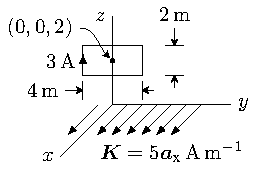
\includegraphics{figInductanceTorqueOnSmallLoopInFieldOfSurfaceCurrent}
\caption{سطحی کثافت برقی رو کے میدان میں بند دائرے پر قوت گردشہ۔}
\end{subfigure}%
%
\begin{subfigure}{0.5\textwidth}
\centering
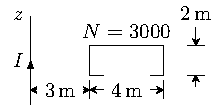
\includegraphics{figInductanceMutualInductanceWireAndRectangularCoil}
\caption{تار اور مستطیل لچھے کی مشترکہ امالہ۔}
\end{subfigure}%
\caption{سوال \حوالہ{سوال_امالہ_سطحی_کثافت_مستطیل_پر_مروڑ} اور سوال \حوالہ{سوال_امالہ_مشترکہ_امالہ_تار_اور_لچھا} کے اشکال۔}
\label{شکل_امالہ_سوالات_سطحی_میدان_اور_دائرہ}
\end{figure}

جوابات:\عددی{\kvec{T}=75.4 \az \, \si{\micro\newton \meter}}، \عددی{\kvec{T}=75.4 \az \, \si{\micro\newton \meter}}
\انتہا{سوال}
%======================
\ابتدا{سوال}
رداس \عددی{\SI{5}{\centi\meter}} کے لمبے پیچدار لچھے میں فی میٹر \عددی{8000} چکر پائے جاتے ہیں۔لچھے میں \عددی{\SI{1.2}{\milli\ampere}} برقی رو گزر رہی ہے۔فی میٹر لچھے میں توانائی \عددی{W} حاصل کریں۔ مساوات \عددی{W=\tfrac{L I^2}{2}} استعمال کرتے ہوئے فی میٹر لچھے کی امالہ حاصل کریں۔

جوابات:\عددی{\SI{0.45}{\micro\joule\per\meter}}، \عددی{\SI{0.631}{\henry\per\meter}}
\انتہا{سوال}
%======================
\ابتدا{سوال}
دو لامحدود لمبائی کے چادر متوازی پڑے ہیں۔ان چادروں پر کثافت برقی رو \عددی{150\ay \, \si{\ampere\per\meter}} اور 
\عددی{-150\ay \, \si{\ampere\per\meter}} ہے۔چادروں کے درمیان لمبا پیچدار لچھا پایا جاتا ہے۔اس لچھے پر \عددی{5000} چکر فی میٹر پائے جاتے ہیں جبکہ اس میں \عددی{\SI{6}{\milli\ampere}} برقی رو گزر رہی ہے۔لچھے کا رداس \عددی{\SI{8}{\centi\meter}} ہے اور اس کا محور \عددی{\ay} سمت میں ہے۔مندرجہ ذیل صورتوں میں لچھے کے فی میٹر لمبائی میں کل توانائی حاصل کریں۔ الف) صرف چادروں میں کثافت برقی رو پائی جاتی ہے۔ ب) صرف لچھے میں برقی رو پائی جاتی ہے۔ پ) چادروں میں کثافت برقی رو اور لچھے میں برقی رو پائی جاتی ہے۔

جوابات:\عددی{\SI{284}{\micro\joule}}، \عددی{\SI{11.4}{\micro\joule}}، \عددی{\SI{296}{\micro\joule}}
\انتہا{سوال}
%=====================
\ابتدا{سوال}
سطح \عددی{x=0} اور \عددی{x=d} پر بالترتیب \عددی{K\az \, \si{\ampere\per\meter}} اور \عددی{-K\az \, \si{\ampere\per\meter}} کثافت برقی رو پائی جاتی ہے۔سطحوں کے درمیان مقناطیسی میدان \عددی{\kvec{H}} حاصل کریں۔چادروں کے درمیان خطہ \عددی{0<y<w}، \عددی{0<z<z_0} میں توانائی \عددی{W} حاصل کریں۔ مساوات \عددی{W=\tfrac{L I^2}{2}} استعمال کرتے ہوئے \عددی{0<y<w} چوڑائی کی فی میٹر امالہ حاصل کریں جہاں \عددی{I} کسی ایک چادر کے \عددی{0<y<w} چوڑائی میں کل برقی رو ہے۔سطح \عددی{y=0} پر چادروں کے درمیان خطہ \عددی{0<z<z0} سے گزرتی کل مقناطیسی بہاو \عددی{\phi} حاصل کریں۔مساوات \عددی{\phi=LI} استعمال کرتے ہوئے فی میٹر امالہ حاصل کریں۔

جوابات:\عددی{K\ay \, \si{\ampere\per\meter}}، \عددی{W=\tfrac{\mu_0}{2} d K^2 w z_0 \, \si{\joule}}، \عددی{L=\tfrac{\mu_0 d}{w}\, \si{\henry\per\meter}}، \عددی{\phi=\mu_0 K d z_0}، \عددی{L=\frac{\mu_0 d}{w} \,\si{\henry\per\meter}}
\انتہا{سوال}
%====================
\ابتدا{سوال}\شناخت{سوال_امالہ_مشترکہ_امالہ_تار_اور_لچھا}
شکل \حوالہ{شکل_امالہ_سوالات_سطحی_میدان_اور_دائرہ}-ب میں \عددی{z} محدد پر پڑی لامحدود لمبائی کے تار میں برقی رو \عددی{I} گزر رہی ہے۔تار کے میدان میں \عددی{3000} چکر کا مستطیل لچھا پایا جاتا ہے۔ان کا مشترکہ امالہ حاصل کریں۔اگر مستطیل کو تین میٹر کے بجائے \عددی{\SI{3}{\milli\meter}} فاصلے پر رکھا جائے تب مشترکہ امالہ کیا حاصل ہو گا۔

جواب:\عددی{\SI{1.02}{\milli\henry}}، \عددی{\SI{8.6}{\milli\henry}}
\انتہا{سوال}
%===============
\ابتدا{سوال}
محدد \عددی{z} پر لامحدود لمبائی کا تار پایا جاتا ہے۔سطح \عددی{x=0} پر ایک چکر کا مربع لچھا پایا جاتا ہے جس کا ایک طرف \عددی{z} محدد کے متوازی اور اس سے \عددی{\SI{1}{\meter}} فاصلے پر ہے۔مربع کے اطراف \عددی{\SI{2}{\meter}} لمبے ہیں۔تار اور لچھے کے مابین مشترکہ امالہ \عددی{M} حاصل کریں۔اگر لچھے کو \عددی{x=0} سطح میں رکھتے ہوئے، \عددی{45^{\circ}} گھمایا جائے تب مشترکہ امالہ کیا ہو گا۔

جوابات:\عددی{\SI{0.439}{\micro\henry}}، \عددی{\SI{0.443}{\micro\henry}}
\انتہا{سوال}
%===============
\ابتدا{سوال}\شناخت{سوال_امالہ_ہم_محوری_تار_بیرونی_تار_اندرونی_امالہ_الف}
صفحہ \حوالہصفحہ{شکل_مقناطیسی_ہم_محوری_تار} میں ہم محوری تار دکھائی گئی ہے۔تصور کریں کہ اس ہم محوری تار کے اندرونی تار میں برقی رو صفر کے برابر ہے جبکہ بیرونی تار میں برقی رو \عددیء{I} کے برابر ہے۔بیرونی تار کی فی میٹر اندرونی امالہ مثال \حوالہ{مثال_امالہ_ہم_محوری_بیرونی_تار_کی_اندرونی_امالہ} کی طرز پر حاصل کریں۔ 

جواب:$\frac{\mu}{2\pi \left(\rho_3^2-\rho_2^2 \right)^2} \left[\rho_2^4 \ln \frac{\rho_3}{\rho_2}+\frac{\rho_3^4-\rho_2^4}{4}-\rho_2^2 \left(\rho_3^2-\rho_2^2\right) \right]$
\انتہا{سوال}
%==========================
\ابتدا{سوال}\شناخت{سوال_امالہ_لامحدود_لمبی_تار}
لامحدود لمبائی کے سیدھی تار کی امالہ مساوات \حوالہ{مساوات_امالہ_مخفی_توانائی_ت} کی مدد سے حاصل کریں۔
\انتہا{سوال}
%================
\ابتدا{سوال}\شناخت{سوال_امالہ_ہم-محوری_بیرونی_تار_اندرونی_ امالہ}
صفحہ \حوالہصفحہ{مثال_امالہ_ہم_محوری_بیرونی_تار_کی_اندرونی_امالہ} پر مثال \حوالہ{مثال_امالہ_ہم_محوری_بیرونی_تار_کی_اندرونی_امالہ} میں ہم محوری تار کے بیرونی تار کی اندرونی امالہ حاصل کی گئی۔اسی کو دوبارہ مساوات \حوالہ{مساوات_امالہ_مخفی_توانائی_ت} کی مدد سے حاصل کریں۔

جواب:بیرونی تار میں \عددیء{H=\tfrac{I}{2\pi \rho}\left(\frac{\rho_3^2-\rho^2}{\rho_3^2-\rho_2^2} \right)} استعمال کرتے ہوئے آگے بڑھیں۔
\انتہا{سوال}
